% ========================================= TEMPLATE INFO ========================================
%
% Author:       P4ntomime
% Version:      1.0.0
% Last updated: 2024-02-18
% Brief:        A LaTeX template for summaries. See README.md for more information.
% 
% ================================================================================================
\documentclass[8pt, a4paper, twoside]{extarticle}
% Font size:    8pt
% Paper size:   A4
% style:        twoside (needed, so odd and even pages have different margins)
% orientation:  portrait. (use 'landscape' for landscape orientation)


% ========================================= DOCUMENT INFO =========================================
\def\title{Funktionen mehrerer Variablen}                               % title
\def\shorttitle{FuVar}                                                  % short title (displayed as PDF title)
\def\dozent{Prof. Dr. Bernhard Zgraggen}                                % lecturer
\def\semester{FS 2024}                                                  % semester
\def\author{Laurin Heitzer, \\Flurin Brechbühler, \\Luca Loop}          % author(s)
\def\repo{https://github.com/P4ntomime/funktionen-mehrerer-variablen}   % repository link
\def\version{1.0.\today}                                                % version
\def\pagelimit{12}                                                      % page limit -> causes pages after limit to be red


% ================================= PACKAGES, SETUP AND COMMANDS ==================================
% =========================================== PACKAGES ============================================
\usepackage[utf8]{inputenc}         % input encoding: UTF-8
\usepackage[T1]{fontenc}            % font encoding: T1
\usepackage{textcomp}               % additional symbols
\usepackage{times}                  % times new roman font
\usepackage[main=ngerman]{babel}    % set main language to german


\usepackage{multicol}               % provides multicols environment
\usepackage{geometry}               % set page layout


\usepackage{enumitem}               % list customization
\usepackage{outlines}               % easy nested lists
\usepackage{tabularx}               % some nicer tables with X columns
\usepackage{multirow}               % multirow in tables
\usepackage{hhline}                 % double lines in tables


\usepackage{amsmath}                % math symbols
\usepackage{amssymb}                % more math symbols
\usepackage{mathtools}
\usepackage{mhsetup}
\usepackage{txfonts}
\usepackage[squaren]{SIunits}       % SI-units
\usepackage{bm}                     % bold math symbols
\usepackage{trfsigns}               % needed for "Laplace" symbol (Korrespondenz)
\usepackage{mathrsfs}               % needed for Fourier transform "F"


\usepackage{graphicx}               % include graphics
\usepackage{graphbox}               % needed for aligning images in multicol environment
\usepackage{scalerel}               % scale any objects
\usepackage{anyfontsize}            % set any font size
\usepackage{xcolor}                 % needed for colors


\usepackage{tcolorbox}              % colored boxes
\usepackage{contour}                % contour for text (used in custom underline command)
\usepackage[normalem]{ulem}         % custom underline (used in custom underline command)


\usepackage{tikz}                   % needed for TikZ drawings


% \usepackage{listings}               % for nicer code display
% to use nodes inside listing see: https://texample.net/tikz/examples/tikz-listings/


\usepackage{hyperref}               % clickable links
\usepackage{qrcode}                 % QR code generation (also clickable)


\usepackage{ifthen}                 % if-then-else commands
\usepackage{calc}                   % simple arithmetic in LaTeX commands


\usepackage{draftwatermark}         % watermark on pages after a certain limit
\usepackage{fancyhdr}               % custom header and footer
\usepackage[explicit]{titlesec}     % custom section titles


\usepackage{datetime2}              % custom date format for versioning


% ========================================== BASIC SETUP ==========================================

% --------------------------------------- DOCUMENT SETTINGS ---------------------------------------
\hypersetup{hidelinks,
% set pdf metadata
            pdfauthor={\author},
            pdftitle={\shorttitle},
            pdfsubject={\title\ \semester},
            pdfkeywords={Gahn go lerne!!}}

% set style for URLs
\urlstyle{same} % sets url font to the same as the preceeding text

% set page layout
\geometry{left=3mm, 
          right=3mm, 
          top=3mm, 
          bottom=6mm, 
          headheight=0mm, 
          headsep=0mm, 
          footskip=4mm}

\setlength{\columnsep}{1.5mm}       % distance between columns
\setlength{\columnseprule}{0.1pt}   % thickness of column separation line
\setlength{\parindent}{0pt}         % no paragraph indentation

\setcounter{tocdepth}{2}            % only display sections and subsections in toc
% \setcounter{secnumdepth}{0}       % uncomment to disable section numbering

\DeclareMathSizes{8}{8}{6}{4}       % set math font sizes for 8pt document


% --------------------------------------- COLOR DEFINITIONS ---------------------------------------
\definecolor{sectioncolor}{HTML}{8acafc}
\definecolor{subsectioncolor}{HTML}{c3e3fd}
\definecolor{sectextcol}{HTML}{000000}
\definecolor{subsectextcol}{HTML}{000000}

\definecolor{backcolour}{HTML}{f5f5f0} % background color for highlighted text

% TODO: define color palette
% color palette: https://colorkit.co/color-palette-generator/FF8552-9e22bd-404E7C-C32E15-225A28/
\definecolor{green}{HTML}{1af430}
\definecolor{red}{HTML}{f90d09}
\definecolor{blue}{HTML}{093ce5}
\definecolor{orange}{HTML}{f7730e}
\definecolor{violet}{HTML}{a516c9}

% colors for listings (code)
% \definecolor{commentcolour}{HTML}{404E7C}
% \definecolor{keywordcolour}{HTML}{225A28}
% \definecolor{stringcolour}{HTML}{9e22bd}
% \definecolor{numbercolour}{HTML}{808080}


% ----------------------------------- LIST AND TABULAR SETTINGS -----------------------------------
\setlist[enumerate]{label=\bfseries\arabic*.,   % label style bold arabic numerals (1., 2., ...)
                    leftmargin=*}               % remove left margin from enumerate
\setlist[itemize]{leftmargin=1.5em}             % left margin for itemize: 1.5em
\setlist{nosep}                                 % no vertical spacing between list items

\renewcommand{\arraystretch}{1.2}               % stretch table rows


% ----------------------------------------- TIKZ SETTINGS -----------------------------------------
\usetikzlibrary{arrows}
\usetikzlibrary{arrows.meta}
\usetikzlibrary{bending}
\usetikzlibrary{decorations.pathreplacing}
\usetikzlibrary{angles}
\usetikzlibrary{tikzmark}
\usetikzlibrary{petri}
\usetikzlibrary{positioning}
\usetikzlibrary{shapes}
\usetikzlibrary{calc}
\usetikzlibrary{fit}


% ------------------------------------ OTHER PACKAGE SETTINGS -------------------------------------

% define and set new date style for versioning as YYYYMMDD
\DTMnewdatestyle{vnumdate}{%
    \renewcommand{\DTMdisplaydate}[4]{\number##1\DTMtwodigits{##2}\DTMtwodigits{##3}}%
    \renewcommand{\DTMDisplaydate}{\DTMdisplaydate}%
}
\DTMsetdatestyle{vnumdate}


% setup for ulem and contour packages
\renewcommand{\ULdepth}{1.75pt} % set underline depth
\contourlength{0.7pt}           % set contour length


% ====================================== SETUP AND COMMANDS =======================================

% custom underline command for exclusions on lowercase letters such as g, j, p, q, y
\newcommand{\myul}[1]{%
    \uline{\phantom{#1}}%
    \llap{\contour*{white}{#1}}%
}


% setup header and footer
\pagestyle{fancy}
\fancyhf{}                          % clear all header and footer fields
\renewcommand{\headrulewidth}{0pt}  % remove header rule
\renewcommand{\footrulewidth}{0pt}  % remove footer rule
\fancyfoot[C]{\thepage}             % page number in center of footer


% --------------------------------------- TITLE FORMATTING ----------------------------------------

% section formatting
\titleformat{\section}
            % {\fontsize{9}{8}\selectfont\bfseries}
            {\Large\bfseries}
            {}
            {0mm}
            {\tikz{
                \node[fill=sectioncolor,            % fill color:       sectioncolor
                      text=sectextcol,              % text color:       sectextcol
                      text width=\columnwidth-4pt,  % text width:       columnwidth - 2x padding
                      text depth=0pt,               % text depth:       0pt (needed so text stays vertically centered)
                      minimum height=5mm,           % minimum height:   5mm
                      inner sep=2pt,                % inner padding:    2pt
                      align=left]                   % text alignment:   left
                      {\thesection\ #1};}}

\titleformat{name=\section, numberless}
            % {\fontsize{9}{8}\selectfont\bfseries}
            {\Large\bfseries}
            {}
            {0mm}
            {\tikz{
                \node[fill=sectioncolor,            % fill color:       sectioncolor
                      text=sectextcol,              % text color:       sectextcol
                      text width=\columnwidth-4pt,  % text width:       columnwidth - 2x padding
                      text depth=0pt,               % text depth:       0pt (needed so text stays vertically centered)
                      minimum height=5mm,           % minimum height:   5mm
                      inner sep=2pt,                % inner padding:    2pt
                      align=left]                   % text alignment:   left
                      {#1};}}

\titlespacing{\section}
             {0mm}
             {.8ex}
             {.8ex}


% subsection formatting
\titleformat{\subsection}
            {\large\bfseries}
            {}
            {0mm}
            {\phantomsection\tikz{
                \node[fill=subsectioncolor,         % fill color:       subsectioncolor 
                      text=subsectextcol,           % text color:       subsectextcol 
                      text width=\columnwidth-4pt,  % text width:       columnwidth - 2x padding 
                      text depth=0pt,               % text depth:       0pt (needed so text stays vertically centered)
                      minimum height=5mm,           % minimum height:   5mm 
                      inner sep=2pt,                % inner padding:    2pt 
                      align=left]                   % text alignment:   left
                      {\thesubsection\ #1};}}

\titleformat{name=\subsection, numberless}
            {\large\bfseries}
            {}
            {0mm}
            {\phantomsection\tikz{
                \node[fill=subsectioncolor,         % fill color:       subsectioncolor 
                      text=subsectextcol,           % text color:       subsectextcol 
                      text width=\columnwidth-4pt,  % text width:       columnwidth - 2x padding 
                      minimum height=5mm,           % minimum height:   5mm 
                      inner sep=2pt,                % inner padding:    2pt 
                      align=left]                   % text alignment:   left
                      {#1};}}

\titlespacing{\subsection}
             {0mm}
             {.8ex}
             {.8ex}


% subsubsection formatting
\titleformat{\subsubsection}
            {\fontsize{10}{9}\selectfont\bfseries}
            % {\fontsize{9}{8}\selectfont\bfseries}
            % {\normalsize\bfseries}
            {\hspace{2pt}\myul{\thesubsubsection\ }}
            {0mm}
            {\phantomsection{}\myul{#1}}

\titlespacing{\subsubsection}
             {0mm}
             {.8ex}
             {.8ex}


% custom command for examples
\newcommand{\example}[1]{\subsubsection*{Beispiel: #1}}


% ----------------------------------- CUSTOM TABULAR SPECIFIERS -----------------------------------

% centered fixed width column type
\newcolumntype{P}[1]{>{\centering\arraybackslash}p{#1}}

 % centered variable width column type
\newcolumntype{C}{>{\centering\arraybackslash}X}

% centered math column type
\newcolumntype{M}{>{$}c<{$}}

% right aligned math column type
\newcolumntype{O}{>{$}r<{$}}


% inline tikz node for later referencing
\newcommand{\tikznode}[2]{% from https://tex.stackexchange.com/a/402466/121799
	\ifmmode%
	\tikz[remember picture,baseline= (#1.base),inner sep=0pt] \node(#1){$#2$};
	\else
	\tikz[remember picture,baseline= (#1.base),inner sep=0pt] \node(#1){#2};
	\fi}


% custom inline tcolorbox
\newtcbox{\mybox}
            [1]
            [backcolour]
            {on line,
            arc=0pt,
            outer arc=0pt,
            colback=#1,
            colframe=#1,
            boxsep=0pt,
            left=1pt,
            right=1pt,
            top=1pt,
            bottom=1pt,
            boxrule=0pt}


\makeatletter

% ------------------------------- SECTIONING COMMANDS CUSTOMIZATION -------------------------------

% section: add optional argument to command for script page numbers
\let\old@sec\section%
\RenewDocumentCommand{\section}{somg}{%
    \IfBooleanTF{#1}{
        \IfNoValueTF{#2}{
            \IfNoValueTF{#4}{
                \old@sec*{#3}
            }{
                \old@sec*{#3 {\small(S. #4)}}
            }
        }{
            \IfNoValueTF{#4}{
                \old@sec*[#2]{#3}
            }{
                \old@sec*[#2]{#3 {\small(S. #4)}}
            }
        }%
    }{
        \IfNoValueTF{#2}{
            \IfNoValueTF{#4}{
                \old@sec{#3}
            }{
                \old@sec{#3 {\small(S. #4)}}
            }
        }{
            \IfNoValueTF{#4}{
                \old@sec[#2]{#3}
            }{
                \old@sec[#2]{#3 {\small(S. #4)}}
            }
        }%
    }
}


% subsection: add optional argument to command for script page numbers
\let\old@subsec\subsection%
\RenewDocumentCommand{\subsection}{somg}{%
    \IfBooleanTF{#1}{
        \IfNoValueTF{#2}{
            \IfNoValueTF{#4}{
                \old@subsec*{#3}
            }{
                \old@subsec*{#3 {\small(S. #4)}}
            }
        }{
            \IfNoValueTF{#4}{
                \old@subsec*[#2]{#3}
            }{
                \old@subsec*[#2]{#3 {\small(S. #4)}}
            }
        }%
    }{
        \IfNoValueTF{#2}{
            \IfNoValueTF{#4}{
                \old@subsec{#3}
            }{
                \old@subsec{#3 {\small(S. #4)}}
            }
        }{
            \IfNoValueTF{#4}{
                \old@subsec[#2]{#3}
            }{
                \old@subsec[#2]{#3 {\small(S. #4)}}
            }
        }%
    }
}


% subsubsection: add optional argument to command for script page numbers
\let\old@subsubsec\subsubsection%
\RenewDocumentCommand{\subsubsection}{somg}{%
    \IfBooleanTF{#1}{
        \IfNoValueTF{#2}{
            \IfNoValueTF{#4}{
                \old@subsubsec*{#3}
            }{
                \old@subsubsec*{#3 {\small(S. #4)}}
            }
        }{
            \IfNoValueTF{#4}{
                \old@subsubsec*[#2]{#3}
            }{
                \old@subsubsec*[#2]{#3 {\small(S. #4)}}
            }
        }%
    }{
        \IfNoValueTF{#2}{
            \IfNoValueTF{#4}{
                \old@subsubsec{#3}
            }{
                \old@subsubsec{#3 {\small(S. #4)}}
            }
        }{
            \IfNoValueTF{#4}{
                \old@subsubsec[#2]{#3}
            }{
                \old@subsubsec[#2]{#3 {\small(S. #4)}}
            }
        }%
    }
}


% custom text rightarrow to match tikz arrows
\renewcommand{\textrightarrow}{
    \tikz{
        \draw[-{Stealth[length=1.7mm]},
              double]
                (0,0) to (0.3,0);}}

% custom text leftrightarrow to match tikz arrows
\newcommand{\textlrarrow}{
    \tikz{
        \draw[{Stealth[length=1.7mm]}-{Stealth[length=1.7mm]},
              double]
                (0,0) to (0.4,0);}}


% renews the pmatrix environment to use \lgroup and \rgroup instead of \left( and \right)
\renewenvironment{pmatrix}{%
    \left\lgroup%
    \matrix@check\pmatrix\env@matrix%
}{
    \endmatrix\right\rgroup%
}

% renews the pmatrix* environment to use \lgroup and \rgroup instead of \left( and \right)
\MHInternalSyntaxOn%
\renewenvironment{pmatrix*}[1][c]
  {\left\lgroup\MT_matrix_begin:N #1}
  {\MT_matrix_end:\right\rgroup}
\MHInternalSyntaxOff%


% custom command for size matched colored brackets
\newcommand{\bbr}[2]{\colorlet{saved}{.}\color{#1}\left\lgroup\color{saved}#2\color{#1}\right\rgroup\color{saved}}


% custom command for differential operator d
\newcommand{\diff}{\ensuremath{\mathop{} \! \mathrm{d}}}

\newcommand{\rreal}{\ensuremath{\mathbb{R}}}
\newcommand{\nnatural}{\ensuremath{\mathbb{N}}}

% custom command for underset limes operator
\newcommand{\limes}[1]{\ensuremath{\underset{#1}{\lim}}}

% custom command for absolute value
\newcommand{\abs}[1]{\ensuremath{\left|#1\right|}}


% shortcuts for colored text
\newcommand{\cgn}[1]{{\color{green}#1}}
\newcommand{\crd}[1]{{\color{red}#1}}
\newcommand{\cbl}[1]{{\color{blue}#1}}
\newcommand{\cor}[1]{{\color{orange}#1}}
\newcommand{\cvt}[1]{{\color{violet}#1}}


\newcommand{\warn}[1]{
    \tikz[baseline=($(current bounding box.center)!0.65!(current bounding box.south)$)]{
        \node[isosceles triangle, 
              isosceles triangle stretches, 
              shape border rotate=90, 
              draw=red, 
              text=red,
              semithick,
              inner sep=0mm,
              minimum width=3mm, 
              minimum height=2.5mm, 
              rounded corners=0.5mm] {\bfseries \raisebox{0.1mm}{\footnotesize !}};}\crd{\textbf{ #1}}}

% \newcommand{\warnsymbol}{
%     \hspace{0.5mm}
%     \tikz[baseline=($(current bounding box.center)!0.65!(current bounding box.south)$)]{
%         \node[isosceles triangle, 
%               isosceles triangle stretches, 
%               shape border rotate=90, 
%               draw=red, 
%               text=red,
%               semithick,
%               inner sep=0mm,
%               minimum width=3mm, 
%               minimum height=2.5mm, 
%               rounded corners=0.5mm] {\bfseries \raisebox{0.1mm}{\footnotesize !}};}
% }


\newcommand{\txtqt}[1]{\textquotedbl #1\textquotedbl}

% bullet command for items in tables
\newcommand{\tabitem}{~~\llap{\textbullet}~~}


% customizes watermark and page color after a certain page limit
% colors all pages after the specified limit red
% source: https://stackoverflow.com/questions/2720534/force-a-maximum-number-of-pages-in-latex 
\newcounter{page@count}
\setcounter{page@count}{0}
\gdef\maxpages{\pagelimit}
\ifx\latex@outputpage\@undefined\relax% ChkTeX 21
    \global\let\latex@outputpage\@outputpage% ChkTeX 21
\fi%
\gdef\@outputpage{% ChkTeX 21
    \addtocounter{page@count}{1}%
    \ifnum\value{page@count}>\maxpages\relax%
        % change page background to red and add watermark
        \SetWatermarkText{\pagelimit\ Seiten Limit erreicht!}%
        \SetWatermarkScale{0.35}%
        \pagecolor{red}
        \latex@outputpage%
    \else%
        \SetWatermarkText{}%
        \latex@outputpage%
    \fi%
}


% remove title from table of contents, needed for layout
\renewcommand{\tableofcontents}{%
    \@starttoc{toc}
}


% scale super- and subscript -- not used currently, instead resized math font
% \catcode`_=\active% chktex 41 --> suppress ChkTeX warning
% \catcode`^=\active% chktex 41
% \newcommand_[1]{\ensuremath{\sb{\mathrm{\scaleobj{0.7}{#1}}}}}
% \newcommand^[1]{\ensuremath{\sp{\mathrm{\scaleobj{0.7}{#1}}}}}


\makeatother


% new environment for layout --> automatically adjusts to landscape or portrait
\NewDocumentEnvironment{layout}{}
                            {\ifthenelse{\paperwidth > \paperheight} % ChkTeX 1
                            % LANDSCAPE LAYOUT
                            {\begin{multicols*}{3} % ChkTeX 15
                                \begin{minipage}[t]{0.18\columnwidth}
                                    \vspace{-0.225\columnwidth}
                                    \qrcode[level=L, 
                                            version=0,
                                            height=0.9\columnwidth]{\repo}\\[1mm]
                                    \normalfont\footnotesize V \version{}
                                    \smallskip
                                \end{minipage}\hfill
                                \begin{minipage}[t]{0.81\columnwidth}
                                    \raggedright%
                                    \normalfont\huge\bfseries\title{}\\
                                    \normalfont\Large\semester\ -- \dozent{}\\
                                    \normalfont\large Autoren:\\
                                    \normalfont\large\author{}\\[2mm]
                                \end{minipage}
                                \normalfont\normalsize\myul{\url{\repo}}
                                \raggedcolumns}
                            % PORTRAIT LAYOUT
                            {\hfill\null\vspace{1cm}
                            \begin{center}
                                \normalfont\fontsize{35}{32}\selectfont\bfseries\title{}\\[7.5mm]
                                \normalfont\huge\semester\ \dozent{}\\
                                \normalfont\Large Autoren:\\
                                \normalfont\Large\author{}\\[2mm]
                                \normalfont\large Version:\\
                                \normalfont\large\version{}\\
                                \normalfont\normalsize\myul{\url{\repo}}\\[2mm]
                                \qrcode[level=L, 
                                        version=0,
                                        height=2cm]{\repo}
                            \end{center}
                            \vfill
                            \section*{\contentsname}
                            \begingroup
                            \setlength{\columnsep}{5mm}
                            \begin{multicols}{2}
                                \tableofcontents%
                            \end{multicols}
                            \endgroup
                            \vfill
                            \thispagestyle{empty}
                            \newpage
                            \begin{multicols*}{2}
                            \raggedcolumns}
                         }
                         {\end{multicols*}}


% new environment for centered tabulars
\NewDocumentEnvironment{ctabular}{m}
                        {\center\tabular{#1}}
                        {\endtabular\endcenter}


\NewDocumentEnvironment{rrcases}{}
                        {\left.\begin{aligned}}
                        {\end{aligned}\right\rbrace}
% ---------------------------------------- LISTINGS SETUP -----------------------------------------

% % hack to fix asterisk in lstlisting
% \makeatletter
% \lst@CCPutMacro%
%     \lst@ProcessOther{"2A}{% ChkTeX 18
%          {\raisebox{0.125pt}{*}}}
%     \@empty\z@\@empty% ChkTeX 21
% \makeatother


% % inline lst tikz node for later referencing
% \newcommand{\lstnode}[2][0.5ex]{
% 	\tikz[overlay, remember picture, inner sep=0pt, yshift=#1, minimum width=0mm]\node(#2){};
% }


% custom inline listings with box around them
% \newcommand{\mylstbox}[2][columns=fullflexible]{
%     \mybox{
%         \lstinline[#1]{#2}}}
% \newcommand{\mytclstbox}[2][columns=fullflexible]{
%     \mybox{
%         \lstinline[basicstyle=\sffamily\footnotesize\color{#1}, columns=fullflexible]{#2}}}


% % renew command for lstinputlisting with less vertical spacing
% \renewcommand{\lstinputlisting}[2][]{
%     \begingroup
%     \vspace{-0.6\abovedisplayskip}
%     \lst@setcatcodes%
%     \lst@inputlisting[#1]{#2}
%     \vspace{-0.6\abovedisplayskip}
% }


% % listings style (code)
% \lstdefinestyle{mystyle}{
%     backgroundcolor=\color{backcolour},   
%     commentstyle=\color{commentcolour},
%     keywordstyle=\bfseries\color{keywordcolour},
%     numberstyle=\tiny\color{numbercolour},
%     stringstyle=\color{stringcolour},
%     basicstyle=\sffamily,
%     breakatwhitespace=false,
%     breaklines=true,
%     captionpos=b,
%     keepspaces=true,
%     numbers=left,
%     numbersep=2pt,
%     showspaces=false,
%     showstringspaces=false,
%     showtabs=false,
%     tabsize=4,
% 	xleftmargin=1em,
% 	language=Java,
%     extendedchars=true,
%     inputencoding=cp1252,
% 	columns=[l]fullflexible	% see: https://tex.stackexchange.com/questions/99416/latex-source-code-listing-with-less-space-between-characters or manual
% }


% % custom lstinline command with custom colors
% \def\purplst{\begingroup\color{violet}}
% \def\greenlst{\begingroup\color{green}}
% \def\redlst{\begingroup\color{red}}
% \def\ywlst{\begingroup\color{orange}}
% \def\bluelst{\begingroup\color{blue}}
% \def\endlstcol{\endgroup}


% % basic lstinline style without colors
% \lstdefinestyle{basestyle}{
%     backgroundcolor=\color{backcolour},
%     keywordstyle=\bfseries,
%     numberstyle=\tiny\color{numbercolour},
%     basicstyle=\sffamily\footnotesize,
%     breakatwhitespace=false,     
%     breaklines=true,
%     captionpos=b,
%     keepspaces=true,
%     numbers=none,
%     numbersep=2pt,
%     showspaces=false,
%     showstringspaces=false,
%     showtabs=false,
%     tabsize=4,
%     xleftmargin=0em,
%     language=Java,
%     columns=flexible,	% see: https://tex.stackexchange.com/questions/99416/latex-source-code-listing-with-less-space-between-characters or manual
% }


% \lstset{
%     style=mystyle,
%     morekeywords={final, override, enum, var, List, Set, Map, String, Object},
%     moredelim=[il][\textcolor{orange}]{¦¦},
%     moredelim=[is][\textcolor{orange}]{&&}{&&},
%     moredelim=[is][\textcolor{violet}]{@}{@},
% }


% =========================================== DOCUMENT ============================================
\begin{document}
    \begin{layout}
        \section{Dimensionen, Schnitte und Konturen}
        \newpage
\section{Ableitungen, DGL und Gradienten (bi-variat)}
\[
    f:\mathbb{D}_f\subseteq \mathbb{R}^2\rightarrow \mathbb{W}_f\subseteq \mathbb{R}\quad\mathrm{skalar}
\]
\subsection{Partielle Ableitung}
Ableitung einer Partiellen Funktion. 

\example{Bi-Variate Funktion}
\[
    f(x, y):\, y \text{ fixieren} = \text{const.} = y_{0};\quad x \text{ \textbf{einzige} freie Variable}
\]

\subsubsection*{Notationen}

\begin{ctabular}{l l}
    1. Ordnung: & $\displaystyle f(x; y_{0})\Rightarrow \frac{\partial f}{\partial x} = f_{x}(x; y_{0})$ \\
    \multirow{2}*{2. Ordnung:}  &  $\displaystyle \frac{\partial}{\partial x}
                                    \left\lgroup\frac{\partial f}{\partial x}\right\rgroup = 
                                    \frac{\partial^{2}f}{\partial x^{2}} = f_{xx}$\\
                                &  $\displaystyle \frac{\partial}{\partial y}
                                        \left\lgroup\frac{\partial f}{\partial x}\right\rgroup = 
                                    \frac{\partial^{2}f}{\partial y \partial x} = f_{xy}$
\end{ctabular}


\subsubsection{Schwarz-Symmetrie}
Wenn \cor{$f_{xx}, f_{yy}, f_{xy}$ \& $f_{yx}$} \textbf{stetig} (sprungfrei) sind, dann gilt:
\[
    f_{xy} \overset{!}{=} f_{yx}
\]

         
\subsection{Gradient (Nabla-Operator)}\label{section:diff_dgl_gradient_bivar:gradient}
Spaltenvektor mit partiellen Ableitungen
\[
    \tikznode{grad}{\nabla} f = \begin{pmatrix}
        \frac{\partial f^{\mathstrut}}{\partial^{\mathstrut} x}\\
        \frac{\partial f^{\mathstrut}}{\partial^{\mathstrut} y}\\
        \vdots      % TODO: reformat vdots. They look like shit
    \end{pmatrix} \hat{=} \text{Vektorfeld}
\]

% TODO: some TikZ. Might not be needed and could be removed if unnecessary
\begin{tikzpicture}[overlay, remember picture, >={Latex}]
    \node[inner sep=0pt, ellipse, fit=(grad), draw, densely dotted]{};
    \node[below left= 2mm and 5mm of grad] (gtext) {\txtqt{Gradient} / Nabla};
    \draw[->, rounded corners] (gtext.east) -| ($(grad.south)+(0,-1mm)$);
\end{tikzpicture}


\subsection{Totale Ableitung}
Für Fehlerrechnung benützt, da man hierbei die Abstände von $(x; y; z)$ 
zu einem festen Punkt $(x_{0}; y_{0}; z_{0})$ erhält. (relative Koordinaten)

\[
    D(f;\underbrace{(x_{0}, y_{0}, \ldots)}_{\text{Arbeitspunkt}}):\, 
    \rreal^{\tikznode{somea}{\scriptstyle 2}} \rightarrow \rreal^{\tikznode{someb}{\scriptstyle 1}};\, 
    \text{\txtqt{gute Approximation}}
\]
\[
    f(x = x_{0} + \Delta x; y = y_{0} + \Delta y; \ldots) = (D_{11}; D_{12})\cdot \begin{pmatrix}
        \Delta x\\
        \Delta y
    \end{pmatrix} + f(x_{0}; y_{0}) + \cgn{R_{1}}
\]
Wobei \cgn{$R_{1}$} dem \txtqt{Rest} entspricht. (Ähnlich wie bei Taylorreihe)

\begin{minipage}[c]{0.7\columnwidth}
    \[
        \frac{\cgn{R_{1}}}{\cor{d = \sqrt{\Delta x^{2} + \Delta y^{2}}}} \rightarrow 0 \text{ (\txtqt{gut}, \txtqt{schneller gegen 0 als $\cor{d}$})}
    \]
\end{minipage}\hfill
\begin{minipage}[c]{0.29\columnwidth}
    \begin{tikzpicture}[baseline=(current bounding box.center), 
                        >={Latex[width=1mm, 
                                 length=1mm]}, 
                        scale=0.5, 
                        font=\tiny]

        % Koordinatensystem
        \draw[->] (0,0) -- (4,0) node[below]{$x$};
        \draw[->] (0,0) -- (0,2.5) node[left]{$y$};

        % Punkte
        \node[circle, fill=black, inner sep=0pt, minimum size=2pt] (A) at (1.7,0.7) {};
        \node[circle, fill=black, inner sep=0pt, minimum size=2pt] (P) at (0.7,1.7) {};
        \node[inner sep=1pt, right=1mm of A] {$A=(x_{0}; y_{0})$};
        \node[inner sep=1pt, above right=0.1mm and -1ex of P] {$P=(x;y)$};
    
        % Differenz
        \draw (P) -- (A-|P) node[midway, left]{$\Delta y$} -- (A) node[midway, below]{$\Delta x$};
        \draw[orange] (P) -- (A) node[midway, above right, inner sep=1pt]{\cor{$d$}};
    \end{tikzpicture}
\end{minipage}

\[
    \begin{split}
        D(f;(x_{0}; y_{0})) &= \left\lgroup D_{11} = \frac{\partial f}{\partial x}(x_{0}; y_{0}); 
                                            D_{12} = \frac{\partial f}{\partial y}(x_{0}; y_{0})\right\rgroup\\
        &= (\nabla f)^{\tr} \text{ \cbl{wenn $\frac{\partial f}{\partial x}; \frac{\partial f}{\partial y}$ stetig bei $A$}}
    \end{split}
\]

\begin{tikzpicture}[overlay, remember picture]
    \draw[tips, -{Latex}] (someb) to[out=135, in=45, edge node={node[above=0mm]{\tiny $1\times 2$ Matrix}}] (somea);
\end{tikzpicture}


\subsection{Linearapproximation (Tangentialapproximation)}
\[
    f(x;y) \approx f(x_{0}; y_{0}) + D(f;(x_{0}; y_{0}))\cdot \begin{pmatrix}
        \Delta x\\
        \Delta y
    \end{pmatrix}
    \quad\text{ linear in $\Delta x$ und $\Delta y$}
\]


\subsubsection{Tangentialebene}
\[
    \crd{g(x; y) = f(x_{0}; y_{0}) + D(f;(x_{0}; y_{0}))\cdot \begin{pmatrix}
        x - x_{0}\\
        y - y_{0}
    \end{pmatrix}}
\]
\[
    g(x;y)=f(x_0;y_0)+f_x(x_0;y_0)\cdot(x-x_0)+f_y(x_0;y_0)\cdot(y-y_0)
\]

\subsubsection{Tangentialer Anstieg (Totale Differential)}
\[
    \cvt{\diff f \overset{!}{=} 
        \frac{\partial f}{\partial \tikznode{ptx}{x}}\diff x + 
        \frac{\partial f}{\partial \tikznode{pty}{y}}\diff y} 
        \quad \text{bezüglich } A=\underbrace{(x_{0}; y_{0})}_{\tikznode{axy}{}}
\]
\begin{tikzpicture}[overlay, 
                    remember picture, 
                    >={Latex[width=1mm, 
                             length=1mm]}]

    \draw[->] ($(axy)+(0, 1.8mm)$) to[bend left=10] (ptx.south east);
    \draw[->] ($(axy)+(0, 1.8mm)$) to[bend left=10] (pty.south east);
\end{tikzpicture}


\subsubsection{Differential-Trick (\texorpdfstring{$\diff f$}{df} Trick)}
Auf Kontouren sei $\diff f = 0$ (Kontourlinien). Daher lässt sich folgende Gleichung aufstellen:
\[
\begin{aligned}
    f &= c = \mathrm{const.} \quad | \diff(\ldots)\\
    \diff f &= \diff c \overset{!}{=} 0
\end{aligned}
\]
Bzw. für Kontourlinien: $f_{x}\diff x + f_{y}\diff y = 0$


\subsubsection{Implizite (Steigungs-)Funktion}
\begin{minipage}[c]{0.6\columnwidth}
    \[
        \cbl{y'(x)} = \frac{\diff y}{\diff x} = -\frac{f_{x}}{f_{y}\crd{\neq 0}} \lor 
        \cbl{x'(y)} = \frac{\diff x}{\diff y} = -\frac{f_{y}}{f_{x}\crd{\neq 0}}
    \]
\end{minipage}\hfill
\begin{minipage}[c]{0.39\columnwidth}
    \begin{tikzpicture}[>={Latex[width=1mm,
                                 length=1mm]}, 
                        scale=0.75, 
                        font=\small]

        % Koordinatensystem
        \draw[->] (0,0) -- (3,0) node[below]{$x$};
        \draw[->] (0,0) -- (0,2) node[left]{$y$};
        
        % Funktionen
        \draw[color=green] plot[domain=0.55:1.5] (\x, {-((\x-1.5)*(\x-1.5))+1}) node[right]{$y$}; % y = -((x-1.5)^2)+1
        \draw[color=blue] node[above right]{$y'$} plot[domain=0.25:1.5] (\x, {\x-0.25}); % y = x-0.25

        % Arbeitspunkt
        \node[circle, fill=black, inner sep=0pt, minimum size=1.5pt] (P) at (1,0.75) {};
        \node[inner sep=0pt, above left=0.25mm and 0mm of P] {$P_{0}$};
        \draw[gray, dashed] (P) -- (P-|0,0) node[left]{$y_{0}$};
        \draw[gray, dashed] (P) -- (P|-0,0) node[below]{$x_{0}$};

        % Richtungselemente
        \draw[orange, semithick, ->] (P) -- (2,1.75) node[above, midway, rotate=45]{$\vec{r}$};
        \draw[->] (P) -- (P-|2,0) node[midway, below]{$\diff x$};
        \draw[->] (P-|2,0) -- (2,1.75) node[midway, right]{$\diff y$};
    \end{tikzpicture}
\end{minipage}




% \subsection{Differential}


\subsection{DGL}
\[
    y' = \tikznode{rhsfn}{\bbr{violet}{-\frac{f_{x}}{f_{y}}}};\, y(x_{0}) = y_{0}
\]
\begin{tikzpicture}[overlay, 
                    remember picture] 
    \node[below=1mm of rhsfn, inner sep=0pt, font=\tiny, text=violet] {right-hand-side (r.h.s.) Funktion};
\end{tikzpicture}


\subsection{Richtungselement (Tangentiallinie an Kontouren)}
\[
    \vec{r} = \left\lgroup\diff x = h; \diff y = y'\diff x = -\frac{f_{x}}{f_{y}}\diff x\right\rgroup^{\tr}
\]


\subsection{Gradientenfeld \texorpdfstring{$\perp$}{\_|\_} Kontouren}
\[
    \nabla f \tikznode{scprd}{\dotp} \begin{pmatrix}
        \diff x\\
        \diff y = y'\diff x
    \end{pmatrix} \overset{!}{=} 0
\]
\begin{tikzpicture}[overlay,
                    remember picture,
                    >={Latex[width=1mm, 
                             length=1mm]}]
    \node[above left=2mm and 4mm of scprd, inner sep=0pt, anchor=south east] (spnode) {Skalarprodukt};
    \draw[->] (spnode.east) to[out=0, in=90] ($(scprd.north)+(0,0.2mm)$);
\end{tikzpicture}


\subsection{TODO: Taylorreihe}

\begin{tikzpicture}[>={Latex[width=1mm,
                       length=1mm]}]
    \draw[->] (-1,0) -- (3,0) node[below]{$x$};
    \draw[->] (0,-0.5) -- (0,2) node[left]{$y$};

    % Schnitt
    \draw[green] (-1,-0.5) -- (1, 0.75);
\end{tikzpicture}


\begin{ctabular}{r l}
    $s(t) :$    &$P_0 + t \cdot \hat{v} \mid t\in \rreal$\\
    $s(t) :$    &$f(x_0 + t \cdot \hat{v}_1\, ;\, y_0 + t \cdot \hat{v}_2)$\\
    &\\
    $\frac{\diff s(t)}{\diff t}=\dot{s}(t) :$&$t\mapsto\overbrace{\begin{pmatrix}x_0+t\cdot v_1\\y_0+t\cdot v_2\end{pmatrix}}^{\begin{pmatrix}x\\y\end{pmatrix}}\mapsto f(x,y)$
\end{ctabular}


\subsection{Richtungs-Ableitung}
\[
    \frac{\partial f}{\partial\hat{v}}\overset{!}=D(f;(x_{0};y_{0}))\cdot\hat{v}\overset{\text{Def.}}\Leftrightarrow \grad(f)^{\tr}\cdot\hat{v}=f_{x}\cdot v_{1}+f_{y}\cdot v_{2}
\]

\example{Richtungs-Ableitung}

\[
    \vec{x} : \vec{v} = 
\begin{pmatrix}
    1\\
    0
\end{pmatrix}
= \hat{e}_1
\quad\Rightarrow\quad
    \frac{\partial f}{\partial\hat{e}_{1}}=f_{x}\cdot1+f_{y}\cdot0=\uuline{f_{x}\strut}
\]


\subsubsection{Spezialfälle}


\begin{minipage}[c]{.72\columnwidth}
    \begin{outline}
        \1 $\alpha = \frac{\pi}{2}$ \textrightarrow\ rechter Winkel % TODO: fix \pi --> should be upright
        \1 $\frac{\partial f}{\partial \hat{v}}$ extremal
            \2 $\alpha = 0$ (max):   $\nabla f \cdot\hat{v} > 0$ \textrightarrow\ \cbl{$\grad(f)$} liegt auf $\hat{v}$
            \2 $\alpha = \pi$ (min): $\nabla f \cdot\hat{v} < 0$ \textrightarrow\ \cbl{$\grad(f)$} liegt invers auf $\hat{v}$
    \end{outline}
\end{minipage}\hfill
\begin{tikzpicture}[%
    baseline=(current bounding box.center),
    scale=0.75,
    >={Latex[%
        width=1mm, 
        length=1mm]}]
    \coordinate (A) at (0,0);
    \coordinate (B1) at (2,0);
    \coordinate (B2) at (2.4,0);
    \coordinate (C) at (2,0.8);

    \draw[->] (A) -- (B2) node[right]{$\hat{v}$};
    \draw[blue, ->] (A) -- (C) node[above=-1mm]{$\grad(f)$};
    \draw[red, ->] (A) -- (B1) node[midway, below]{$\nabla f \dotp \hat{v}$};

    \draw[gray, densely dashed] (C) -- (B1);

    \draw pic[draw=green, angle radius=10mm, pic text=$\alpha$, pic text options=green] {angle=B1--A--C};
    \draw pic[draw=gray, angle radius=2mm, pic text=. , pic text options=gray] {angle=C--B1--A};

    \fill (A) circle (1pt) node[above]{$P_0$};
\end{tikzpicture}

\para{Trigo} $\nabla f\cdot\hat{v} \land \frac{\partial f}{\partial\hat{v}}$ \textrightarrow\ $\cos(\alpha)\cdot\abs{\cbl{\nabla f}}$


        \newpage
\section{Extrema von Funktionen finden}
\myul{\textbf{Stationäritätsbedingung:}} $\nabla f \stackrel{!}{=} \vec{0}$

\subsection{Extrema von Funktionen zweier Variablen finden}
\begin{enumerate}[itemsep=1ex]
    \item \textbf{Gradient von $f$ Null-setzten und kritische Stellen finden:}

    $\nabla f=
    \begin{pmatrix}
        f_x\\
        f_y
    \end{pmatrix} \stackrel{!}{=}
    \begin{pmatrix}
        0\\
        0
    \end{pmatrix}
    \, \, \, \, \, \,
    \Rightarrow 
    \begin{matrix}
        f_{x}=0\\
        f_{y}=0
    \end{matrix}
    \, \, \, \, \, \,
    \Rightarrow
    x_0 \text{ und } y_0 \text{ bestimmen}$

    \item \textbf{Zweite Partielle Ableitungen bestimmen:}
        
    \begin{tabular}{lll}
        $f_{xx} = \dots$ & $f_{xy} = f_{yx} = \dots$ & $f_{yy} = \dots$ \\
    \end{tabular}

    \item \textbf{Determinante $\Delta$ der Hesse-Matrix H bestimmen:}
    
    $\Delta = f_{xx}(x_0;y_0) \cdot f_{yy}(x_0;y_0) - \left(f_{xy}(x_0;y_0)\right)^2 $

    \item \textbf{Auswertung:}
    
    \begin{tabular}{lllcl}
        \hline
        $\Delta > 0$ &AND& $f_{xx}(x_0;y_0) < 0$ &$\Longrightarrow$& $\text{lokales Maximum}$\\
        \hline
        $\Delta > 0$ &AND& $f_{yy}(x_0;y_0) < 0$ &$\Longrightarrow$& $\text{lokales Maximum}$\\
        \hline
        $\Delta > 0$ &AND& $f_{xx}(x_0;y_0) > 0$ &$\Longrightarrow$& $\text{lokales Minimum}$\\
        \hline
        $\Delta > 0$ &AND& $f_{yy}(x_0;y_0) > 0$ &$\Longrightarrow$& $\text{lokales Minimum}$\\
        \hline
        $\Delta < 0$ &&&$\Longrightarrow$& $\text{Sattelpunkt}$\\
        \hline
        $\Delta = 0$ &&&?& $\text{Multi-variate-Taylor-logik ...}$\\
        \hline
    \end{tabular}

\end{enumerate}

\subsection{Extrema von Funktionen mehrerer Variablen finden}

\begin{enumerate}[itemsep=1ex]
    \item \textbf{Gradient von $f$ Null-setzten und kritische Stellen finden:}
    
    $\nabla f=
    \begin{pmatrix}
        f_x\\
        f_y\\
        \vdots \\
        f_t
    \end{pmatrix} \stackrel{!}{=}
    \begin{pmatrix}
        0\\
        0\\
        \vdots \\
        0
    \end{pmatrix}
    \quad \Rightarrow x_0$, $y_0$, $\ldots$, $t_0$ bestimmen
    
    \item \textbf{Zweite Partielle Ableitungen für Hesse-Matrix H bestimmen:}
    
    \begin{minipage}[t]{0.48\columnwidth}
        $\mathbf{H}=\begin{pmatrix}
            f_{xx}&f_{xy}&\ldots &f_{xt}\\
            f_{yx}&f_{yy}&\ldots&f_{yt}\\
            \vdots &\vdots &\ddots &\vdots \\
            f_{tx}&f_{ty}&\ldots&f_{tt}
        \end{pmatrix}$
    \end{minipage}\hfill
    \begin{minipage}[c]{0.48\columnwidth}
        \begin{itemize}
            \item Symmetrien beachten!
            \item Nicht doppelt rechnen!
            \item[] \textrightarrow\ $f_{xt} = f_{tx}$
        \end{itemize}
    \end{minipage}

    \item \textbf{Hesse-Matrix H mit gefundenen Stellen füllen:}

    $\mathbf{H}(x_0,y_0,\ldots t_0)=
    \begin{pmatrix}
        f_{xx}(x_0,y_0,\ldots t_0)&f_{xy}(x_0,y_0, \ldots t_0)&\cdots &f_{xt}(x_0,y_0,\ldots t_0)\\
        f_{yx}(x_0,y_0,\ldots t_0)&f_{yy}(x_0,y_0, \ldots t_0)&\cdots &f_{yt}(x_0,y_0,\ldots t_0)\\
        \vdots &\vdots &\ddots &\vdots \\
        f_{tx}(x_0,y_0,\ldots t_0)&f_{ty}(x_0,y_0, \ldots t_0)&\cdots &f_{tt}(x_0,y_0,\ldots t_0)\end{pmatrix}$

    \item \textbf{Eigenwerte $\lambda_i$ der Hesse-Matrix bestimmen:}

    $\text{det}\left(\mathbf{H}(x_0,y_0,\ldots t_0) - \lambda \cdot \mathbf{E}\right)  = 0$

    Nullstellen $\lambda_i$ finden $\rightarrow  $ Eigenwerte

    \medskip
    \myul{Zur Erinnerung:}\\
    $\mathbf{E} = \begin{pmatrix}
        1&0&\ldots &0\\
        0&1&\ldots&0\\
        \vdots &\vdots &\ddots &\vdots \\
        0&0&\ldots&1\\
    \end{pmatrix}
    , \quad
    \lambda \cdot \mathbf{E} = \begin{pmatrix}
        \lambda&0&\ldots &0\\
        0&\lambda&\ldots&0\\
        \vdots &\vdots &\ddots &\vdots \\
        0&0&\ldots&\lambda\\
    \end{pmatrix}$

    \medskip
    $\mathbf{H}(x_0,y_0,\ldots t_0) - \lambda \cdot \mathbf{E} = \ldots \\
    \ldots  = 
    \begin{pmatrix}
        f_{xx}(x_0,y_0,\ldots t_0)- \lambda&f_{xy}(x_0,y_0, \ldots t_0)&\cdots &f_{xt}(x_0,y_0,\ldots t_0)\\
        f_{yx}(x_0,y_0,\ldots t_0)&f_{yy}(x_0,y_0, \ldots t_0)- \lambda&\cdots &f_{yt}(x_0,y_0,\ldots t_0)\\
        \vdots &\vdots &\ddots &\vdots \\
        f_{tx}(x_0,y_0,\ldots t_0)&f_{ty}(x_0,y_0, \ldots t_0)&\cdots &f_{tt}(x_0,y_0,\ldots t_0)- \lambda\end{pmatrix}$

    \item \textbf{Auswertung:}
    
    \begin{tabular}{lll}
        \hline
        $\lambda_i < 0 \,\,\,\forall i$ &$\Longrightarrow$& $\text{lokales Maximum}$\\
        \hline
        $\lambda_i > 0 \,\,\,\forall i$ &$\Longrightarrow$& $\text{lokales Minimum}$\\
        \hline
        $\lambda_i > 0\,$ und $\,\lambda_i < 0$ &$\Longrightarrow$& $\text{Sattelpunkt}$\\
        \hline
    \end{tabular}

    \medskip
    Erklärung:
    \begin{itemize}
        \item $\lambda_i < 0 \,\,\,\forall i$ $\Leftrightarrow $ Alle $\lambda_i$ sind negativ
        \item $\lambda_i > 0 \,\,\,\forall i$ $\Leftrightarrow $ Alle $\lambda_i$ sind positiv
    \end{itemize}
\end{enumerate}


\subsection{Lokales oder Globales Extremum}
Für eine beliebige die Funktion $f(x, y, \ldots  , t)$ gilt:

$\boxed{\begin{array}{llll}
    f(x,y,\ldots ,t)\leq M_{\max}&\forall(x,y,\ldots ,t)\in\mathbb{D}_f&\Rightarrow&\text{globales Maxinum}\\
    f(x,y,\ldots ,t)>M_{\max}&\exists(x,y,\ldots ,t)\in\mathbb{D}_f&\Rightarrow&\text{kein globales Maximum}\\
    \hline f(x,y,\ldots ,t)\geq M_{\min}&\forall(x,y,\ldots ,t)\in\mathbb{D}_f&\Rightarrow&\text{globales Minimum}\\
    f(x,y,\ldots ,t)<M_{\min}&\exists(x,y,\ldots ,t)\in\mathbb{D}_f&\Rightarrow&\text{kein globales Minimum}
\end{array}}$

\medskip
\begin{tabular}{ll}
    $M_{\max}$: &\text{grösstes lokales Maximum}\\
    $M_{\min}$: &\text{kleinstes lokales Minimum}
\end{tabular}




\subsection{Extrema von Funktionen zweier Variablen mit NB finden}

\begin{enumerate}[itemsep=1ex]
    \item \textbf{Nebenbedingung (NB) in Standartform bringen:}\\
    \begin{minipage}[t]{0.4\linewidth}
        Standartform: $n(x, y) \stackrel{!}{=} 0$
    \end{minipage}\hfill
    \begin{minipage}[t]{0.58\linewidth}
            \textcolor{gray}{Nebenbedingung: $x + y = 1$}\\
            \textcolor{gray}{Standartform der Nebenbedingung: $x + y - 1 = 0$}
    \end{minipage}


    \item \textbf{Lagrancge-Funktion $\mathcal{L}$ aufstellen:}\\
    $\mathcal{L}(x, y, \lambda) =
    f(x, y) + \lambda \cdot n(x, y) \,\,\,\,\,\,$ \textcolor{gray}{Am besten gleich ausmultiplizieren}
    

    \item \textbf{Gradient der Lagrancge-Funktion $\mathcal{L}$ Null-setzten und kritische Stellen finden:}\\
    $\nabla \mathcal{L}=
    \begin{pmatrix}
        \mathcal{L}_x\\
        \mathcal{L}_y\\
        \mathcal{L}_\lambda
    \end{pmatrix} \stackrel{!}{=}
    \begin{pmatrix}
        0\\
        0\\
        0
    \end{pmatrix}
    \, \, \, \, \, \,
    \Rightarrow 
    x_0 \text{ und } y_0 \text{ bestimmen}$
    \hfill

    \item \textbf{Zweite Partielle Ableitungen bestimmen:}\\
    \begin{minipage}[t]{0.4\linewidth}
        $\begin{aligned}
            \mathcal{L}_{\lambda \lambda} &\stackrel{!}{=} 0\\
            \mathcal{L}_{xx} &= \dots\\
            \mathcal{L}_{yy} &= \dots\\
        \end{aligned}$
    \end{minipage}\hfill
    \begin{minipage}[c]{0.58\linewidth}
        $\begin{aligned}
            \mathcal{L}_{\lambda x} &= \mathcal{L}_{x\lambda} = n_x = \dots\\
            \mathcal{L}_{\lambda y} &= \mathcal{L}_{y\lambda} = n_y =\dots\\
            \mathcal{L}_{xy} &= \mathcal{L}_{yx} = \dots\\
        \end{aligned}$
    \end{minipage}


    \item \textbf{Geränderte Hesse Matrix $\overline{\mathbf{H}}$ aufstellen und kritische Stellen einsetzen:}
    
    \begin{tabular}{lll}
        $\overline{\mathbf{H}}(x_0,y_0)$ &$=$&
        $\left(
            \begin{matrix}
                {{\mathcal{L}_{\lambda\lambda}(x_0, y_0)}}&{{\mathcal{L}_{\lambda x}(x_0, y_0)}}&{{\mathcal{L}_{\lambda y}(x_0, y_0)}}\\
                {{\mathcal{L}_{x\lambda}(x_0, y_0)}}&{{\mathcal{L}_{xx}(x_0, y_0)}}&{{\mathcal{L}_{xy}(x_0, y_0)}}\\
                {{\mathcal{L}_{y\lambda}(x_0, y_0)}}&{{\mathcal{L}_{yx}(x_0, y_0)}}&{{\mathcal{L}_{yy}(x_0, y_0)}}\\
            \end{matrix}
        \right)$\\
        &$=$&
        $\left(
            \begin{matrix}
                {{0}}&{{n_{x}(x_0, y_0)}}&{{n_{y}(x_0, y_0)}}\\
                {{n_{x}(x_0, y_0)}}&{{\mathcal{L}_{xx}(x_0, y_0)}}&{{\mathcal{L}_{xy}(x_0, y_0)}}\\
                {{n_{y}(x_0, y_0)}}&{{\mathcal{L}_{yx}(x_0, y_0)}}&{{\mathcal{L}_{yy}(x_0, y_0)}}\\
            \end{matrix}
        \right)$
        
    \end{tabular}


    \item \textbf{Determinante der geränderten Hesse Matrix bestimmen:}\\
    $\text{det}\left(\overline{\mathbf{H}}\right) = ... $

    \item \textbf{Auswertung}\\
    \begin{tabular}{lll}
        \hline
        $\text{det}\left(\overline{\mathbf{H}}\right) > 0$ &$\Longrightarrow$& $\text{lokales Maximum}$\\
        \hline
        $\text{det}\left(\overline{\mathbf{H}}\right) < 0$ &$\Longrightarrow$& $\text{lokales Minimum}$\\
        \hline
        $\text{det}\left(\overline{\mathbf{H}}\right) = 0$ &$\Longrightarrow$& $\text{keine Aussage möglich}$\\
        \hline
    \end{tabular}

\end{enumerate}

\subsection{Extrema von Funktionen mehrerer Variablen mit NB finden}

\begin{enumerate}[itemsep=1ex]
    \item \textbf{Nebenbedingung (NB) in Standartform bringen:}\\
    \begin{minipage}[t]{0.4\columnwidth}
        Standartform: $n(x, y, ... , t) \stackrel{!}{=} 0$
    \end{minipage}\hfill
    \begin{minipage}[t]{0.6\columnwidth}
    \end{minipage}


    \item \textbf{Lagrancge-Funktion $\mathcal{L}$ aufstellen:}\\
    $\mathcal{L}(x, y, ..., t, \lambda) =
    f(x, y, ..., t) + \lambda \cdot n(x, y, ..., t) \,\,\,\,\,\,$ \textcolor{gray}{Am besten gleich ausmultiplizieren}
    

    \item \textbf{Gradient der Lagrancge-Funktion $\mathcal{L}$ Null-setzten und kritische Stellen finden:}
    $\nabla \mathcal{L}=
    \begin{pmatrix}
        \mathcal{L}_x\\
        \mathcal{L}_y\\
        \vdots \\
        \mathcal{L}_t\\
        \mathcal{L}_\lambda
    \end{pmatrix} \stackrel{!}{=}
    \begin{pmatrix}
        0\\
        0\\
        \vdots \\
        0\\
        0
    \end{pmatrix}
    \, \, \, \, \, \,
    \Rightarrow 
    x_0 \text{, } y_0 \text{, }... \text{, } t_0 \text{ bestimmen}$
    \hfill

    \item \textbf{Zweite Partielle Ableitungen bestimmen:}
    

    \begin{tabular}{lllll}
        $\begin{matrix}
        \mathcal{L}_{\lambda \lambda} \stackrel{!}{=} 0\\
        \mathcal{L}_{xx} = \dots\\
        \mathcal{L}_{yy} = \dots\\
        \vdots \\
        \mathcal{L}_{tt} = \dots\\
        \end{matrix}$
        &$\,\,\,\,\,\,\,\,$&
        $\begin{matrix}
        \mathcal{L}_{\lambda x} = \mathcal{L}_{x\lambda} = n_x = \dots\\
        \mathcal{L}_{\lambda y} = \mathcal{L}_{y\lambda} = n_y =\dots\\
        \vdots \\
        \mathcal{L}_{\lambda t} = \mathcal{L}_{t\lambda} = n_t =\dots\\
        \end{matrix}$
        &$\,\,\,\,\,\,\,\,$&
        $\begin{matrix}
        \mathcal{L}_{xy} = \mathcal{L}_{yx}\\
        \mathcal{L}_{xt} = \mathcal{L}_{tx}\\
        \mathcal{L}_{yt} = \mathcal{L}_{ty}\\
        \vdots \\
        \end{matrix}$
    \end{tabular}

    \item \textbf{Geränderte Hesse Matrix $\overline{\mathbf{H}}$ aufstellen und kritische Stellen einsetzen:}\\
    \begin{tabular}{lll}
        $\overline{\mathbf{H}}(\crd{x_0,y_0,\ldots t_0})$ &$=$&
        $\left(
            \begin{matrix}
                {{\mathcal{L}_{\lambda\lambda}(\crd{...})}}&{{\mathcal{L}_{\lambda x}(\crd{...})}}&{{\mathcal{L}_{\lambda y}(\crd{...})}}&{\cdots }&{{\mathcal{L}_{\lambda t}(\crd{...})}}\\
                {{\mathcal{L}_{x\lambda}(\crd{...})}}&{{\mathcal{L}_{xx}(\crd{...})}}&{{\mathcal{L}_{xy}(\crd{...})}}&{\cdots }&{{\mathcal{L}_{xt}(\crd{...})}}\\
                {{\mathcal{L}_{y\lambda}(\crd{...})}}&{{\mathcal{L}_{yx}(\crd{...})}}&{{\mathcal{L}_{yy}(\crd{...})}}&{\cdots }&{{\mathcal{L}_{yt}(\crd{...})}}\\
                {\vdots }&{\vdots }&{\vdots }&{\ddots }&{\vdots }\\
                {{\mathcal{L}_{t\lambda}(\crd{...})}}&{{\mathcal{L}_{tx}(\crd{...})}}&{{\mathcal{L}_{ty}(\crd{...})}}&{\cdots }&{{\mathcal{L}_{tt}(\crd{...})}}\\
            \end{matrix}
        \right)$\\
        &$=$&
        $\left(
            \begin{matrix}
                {{0}}&{{n_{x}(\crd{...})}}&{{n_{y}(\crd{...})}}&{\cdots }&{{n_{t}(\crd{...})}}\\
                {{n_{x}(\crd{...})}}&{{\mathcal{L}_{xx}(\crd{...})}}&{{\mathcal{L}_{\lambda y}(\crd{...})}}&{\cdots }&{{\mathcal{L}_{xt}(\crd{...})}}\\
                {{n_{y}(\crd{...})}}&{{\mathcal{L}_{yx}(\crd{...})}}&{{\mathcal{L}_{yy}(\crd{...})}}&{\cdots }&{{\mathcal{L}_{yt}(\crd{...})}}\\
                {\vdots }&{\vdots }&{\vdots }&{\ddots }&{\vdots }\\
                {{n_{t}(\crd{...})}}&{{\mathcal{L}_{tx}(\crd{...})}}&{{\mathcal{L}_{ty}(\crd{...})}}&{\cdots }&{{\mathcal{L}_{tt}(\crd{...})}}\\
            \end{matrix}
        \right)$
    \end{tabular}

    \item \textbf{Determinante der geränderten Hesse Matrix bestimmen:}\\
    $\text{det}\left(\overline{\mathbf{H}}\right) = ... $

    \item \textbf{Auswertung}\\
    \begin{tabular}{lll}
        \hline
        $\text{det}\left(\overline{\mathbf{H}}\right) > 0$ &$\Longrightarrow$& $\text{lokales Maximum}$\\
        \hline
        $\text{det}\left(\overline{\mathbf{H}}\right) < 0$ &$\Longrightarrow$& $\text{lokales Minimum}$\\
        \hline
        $\text{det}\left(\overline{\mathbf{H}}\right) = 0$ &$\Longrightarrow$& $\text{keine Aussage möglich}$\\
        \hline
    \end{tabular}

\end{enumerate}
        \newpage
\section{Support Vector Machine (SVM)}
Die Support Vector Machine kann verwendet werden, um ein Modell für das Zuordnen von Daten zu entwickeln.
Dadurch wird ein Satz von Punkten, deren Klassifizierung bekannt ist, so linear getrennt, dass der Abstand von der trennenden Geraden zu den beiden Punktegruppen maximal wird.
Es resultiert eine einfache Gleichung, mit der sich neue Daten klassifizieren lassen.

\subsection{Linear Trennbare Daten}
\subsubsection{Allgemeines}

\myul{\textbf{Datenpunkte:}} (2D Beispiel)\\
\begin{tabular}{lllll}
    $A:(\underbrace{(x_1,x_2)}_{\vec{x}_1};y_1)$, &
    $B:(\underbrace{(x_1,x_2)}_{\vec{x}_2};y_2)$, &
    $C:(\underbrace{(x_1,x_2)}_{\vec{x}_3};y_3)$, & 
    $\cdots $, &
    $N:(\underbrace{(x_1,x_2)}_{\vec{x}_n};y_n)$\\
\end{tabular}

$\vec{x}_j$ sind Datenvektoren\\
$y_j$ $\in $ \{$\pm 1$\} klassifiziert die jeweiligen Datenvektoren
\newline
\begin{minipage}[]{0.56\columnwidth}
    \myul{\textbf{Hyperebenen:}}\\
    $\boxed{\vec{w}^{tr}\cdot\vec{x}+b=0}$ \\
    $\vec{w}$: Normalenvektor, $\vec{w} \in \mathbb{R}^d$ und $\vec{w} \neq 0$\\
    $b$: Konstante, $b \in \mathbb{R}$\\
    Dimmension der Hyperebene $= d-1$\\
    Abstand der Hyperebene zum Ursprung: $\frac{\left\lvert b \right\rvert }{\left\lvert \vec{w}\right\rvert }$
    \medskip

    \myul{\textbf{Klassifizierung:}}\\
    $\boxed{\vec{w}^{tr}\cdot\vec{x}+b>0} \Rightarrow \vec{x} $ gehört zur Klasse $y = +1$\\
    $\boxed{\vec{w}^{tr}\cdot\vec{x}+b<0} \Rightarrow \vec{x} $ gehört zur Klasse $y = -1$
    \medskip

    \myul{\textbf{Klassifizierung der Trainigsdaten:}}\\
    $\boxed{\vec{w}^{tr}\cdot\vec{x}_j+b \geq 0} \Rightarrow \vec{x}_j $ gehört zur Klasse $y = +1$\\
    $\boxed{\vec{w}^{tr}\cdot\vec{x}_j+b\leq 0} \Rightarrow \vec{x}_j $ gehört zur Klasse $y = -1$
    \medskip

    \myul{\textbf{Zielfunktion:}}\\
    $\boxed{\frac{2}{\left\lvert \vec{w}\right\rvert }=\frac{2}{w}}$
\end{minipage}\hfill
\begin{minipage}[t]{0.4\columnwidth}
    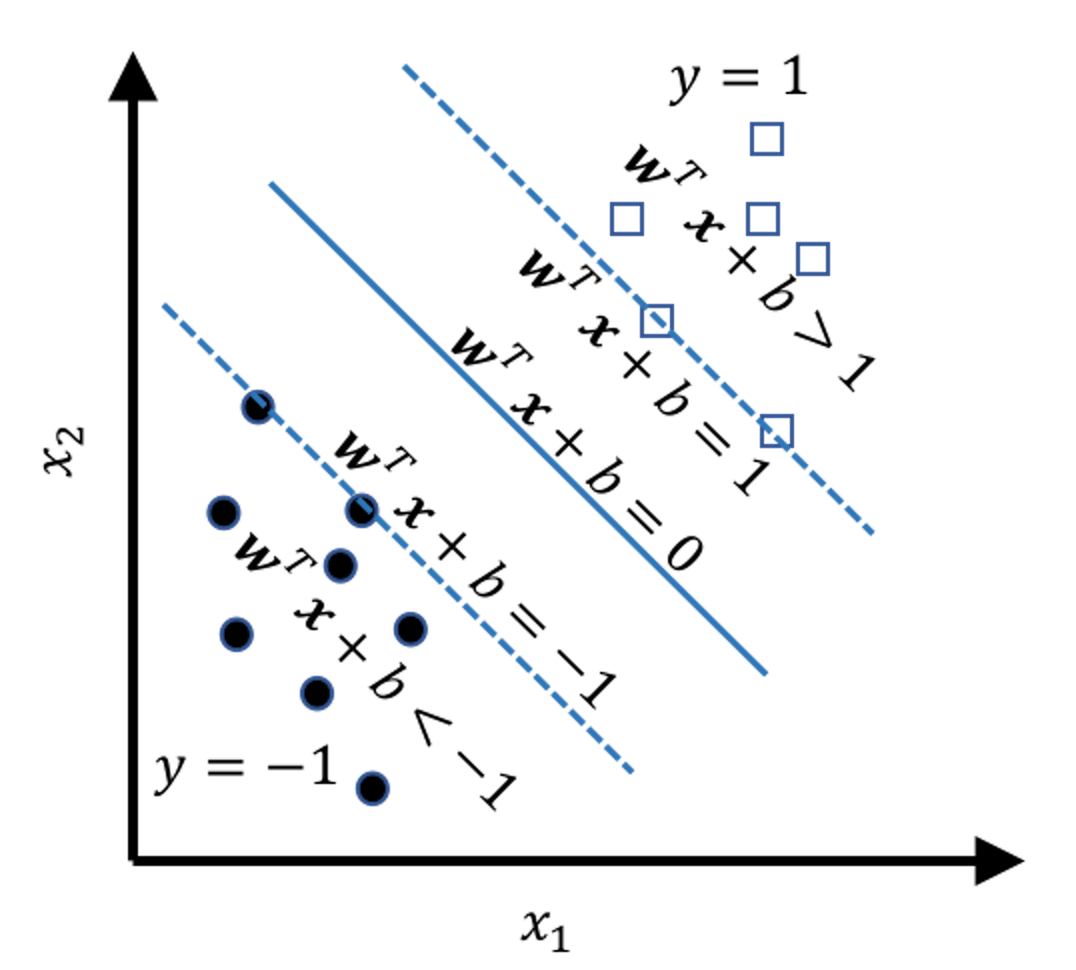
\includegraphics[width=4cm]{images/7_model_values.png}
\end{minipage}

\subsubsection{Das primale Optimierungsproblem}
$\boxed{\frac12\vec{w}^{tr}\cdot\vec{w}=\frac12\left|\vec{w}\right|^2=\frac12w^2\to\min!\quad\mathrm{s.t.}\quad\left(\vec{w}^{tr}\cdot\vec{x}_j+b\right)y_j\geq1\quad\left(j=1,\cdots,N\right)}$

\subsubsection{Das duale Optimierungsproblem}
\myul{\textbf{Nebenbedingung:}}\\
$\boxed{\underbrace{1-\left(\vec{w}^{tr}\cdot\vec{x}_j+b\right)y}_{g_j(\vec{w}^{tr},b)}\leq0\Leftrightarrow g_j(\vec{w}^{tr},b)\leq0\quad\left(j=1,\cdots,N\right)}$
\medskip

\myul{\textbf{Lagrange-Funktion:}}\\
Zusammengesetzt aus dem primalen Problem und den Nebenbedingungen.\\
\begin{tabular}{|r@{ }l|}
    \hline
    $L(\vec{w}^{tr},b,\vec{a})$ & $ =L(w_1,w_2, ...,w_d,b,\alpha_1,\alpha_2, ...,\alpha_N) $ \\
                                & $ =\frac12\vec{w}^{tr}\cdot\vec{w}+\sum_{j=1}^N\alpha_j\left(\underbrace{1-\left(\vec{w}^{tr}\cdot\vec{x}_j+b\right)y_j}_{g_j\left(\vec{w}^{tr},b\right)}\right) $ \\
    \hline
\end{tabular}
\medskip

\myul{\textbf{Stationaritätsbedingungen:}}\\
Aus der Bedingung, dass $\grad(L) = 0$ sein muss, lassen sich folgende Formeln ableiten:
$\boxed{grad_{\left\{\vec{w}^{tr},b\right\}}\left(L(\vec{w}^{tr},b,\vec{\alpha})\right)=\vec{0}} \Leftrightarrow 
\boxed{\vec{w}=\sum_{j=1}^N\alpha_jy_j\vec{x}_j} \text{ und }
\boxed{\sum_{j=1}^N\alpha_jy_j=0}$\\
%\myul{\textbf{Lagrange-Funktion mit den Dualvariablen $\alpha_j$:}}\\
%$\boxed{L(\vec{w}^{tr},b,\vec{\alpha})=\sum_{j=1}^N\alpha_j-\underbrace{\frac12\sum_{j,j'=1}^N\alpha_j\alpha_j,y_jy_j,\vec{x}_j^{tr}\cdot\vec{x}_j}_{\frac{1}{2}\vec{w}^{tr}\cdot\vec{w}}:=L(\vec{\alpha})\quad , \alpha_j\geq0}$
\myul{\textbf{Das duale Problem:}}\\
Die oben erhaltenen Summen können nun in die Lagrange-Fkt. eingesetzt werden. Daraus entsteht\\
$\boxed{L(\vec{\alpha})=\sum_{j=1}^N\alpha_j-\underbrace{\frac12\sum_{j,j'=1}^N\alpha_j\alpha_{j'} \space y_jy_{j'} \space \vec{x}_j^{tr}\cdot\vec{x}_{j'}}_{=\frac12 \vec{w}^{tr} \cdot \vec{w}}\quad\to\quad\max!\quad\mathrm{s.t.}\quad\alpha_j\geq0\wedge\sum_{j=1}^N\alpha_jy_j=0}$

\newcolumn

\myul{\textbf{Vorgehen zum lösen des dualen Optimierungsproblems:}}

\begin{enumerate}
    \item \myul{\textbf{Skizze mit Datenpunkten erstellen:}} \\
    \begin{minipage}[c]{0.6\columnwidth}
        \begin{itemize}
            \item Einzelne Datenpunkte klassenweise farblich hervorheben
            \item Falls ein Datenpunkt der gleichen Klasse weit weg von den anderen ist\\
            \textrightarrow\ diesen vergessen, da sein $\alpha = 0$ sein wird
        \end{itemize}
    \end{minipage}\hfill
    \begin{minipage}[c]{0.33\columnwidth}
        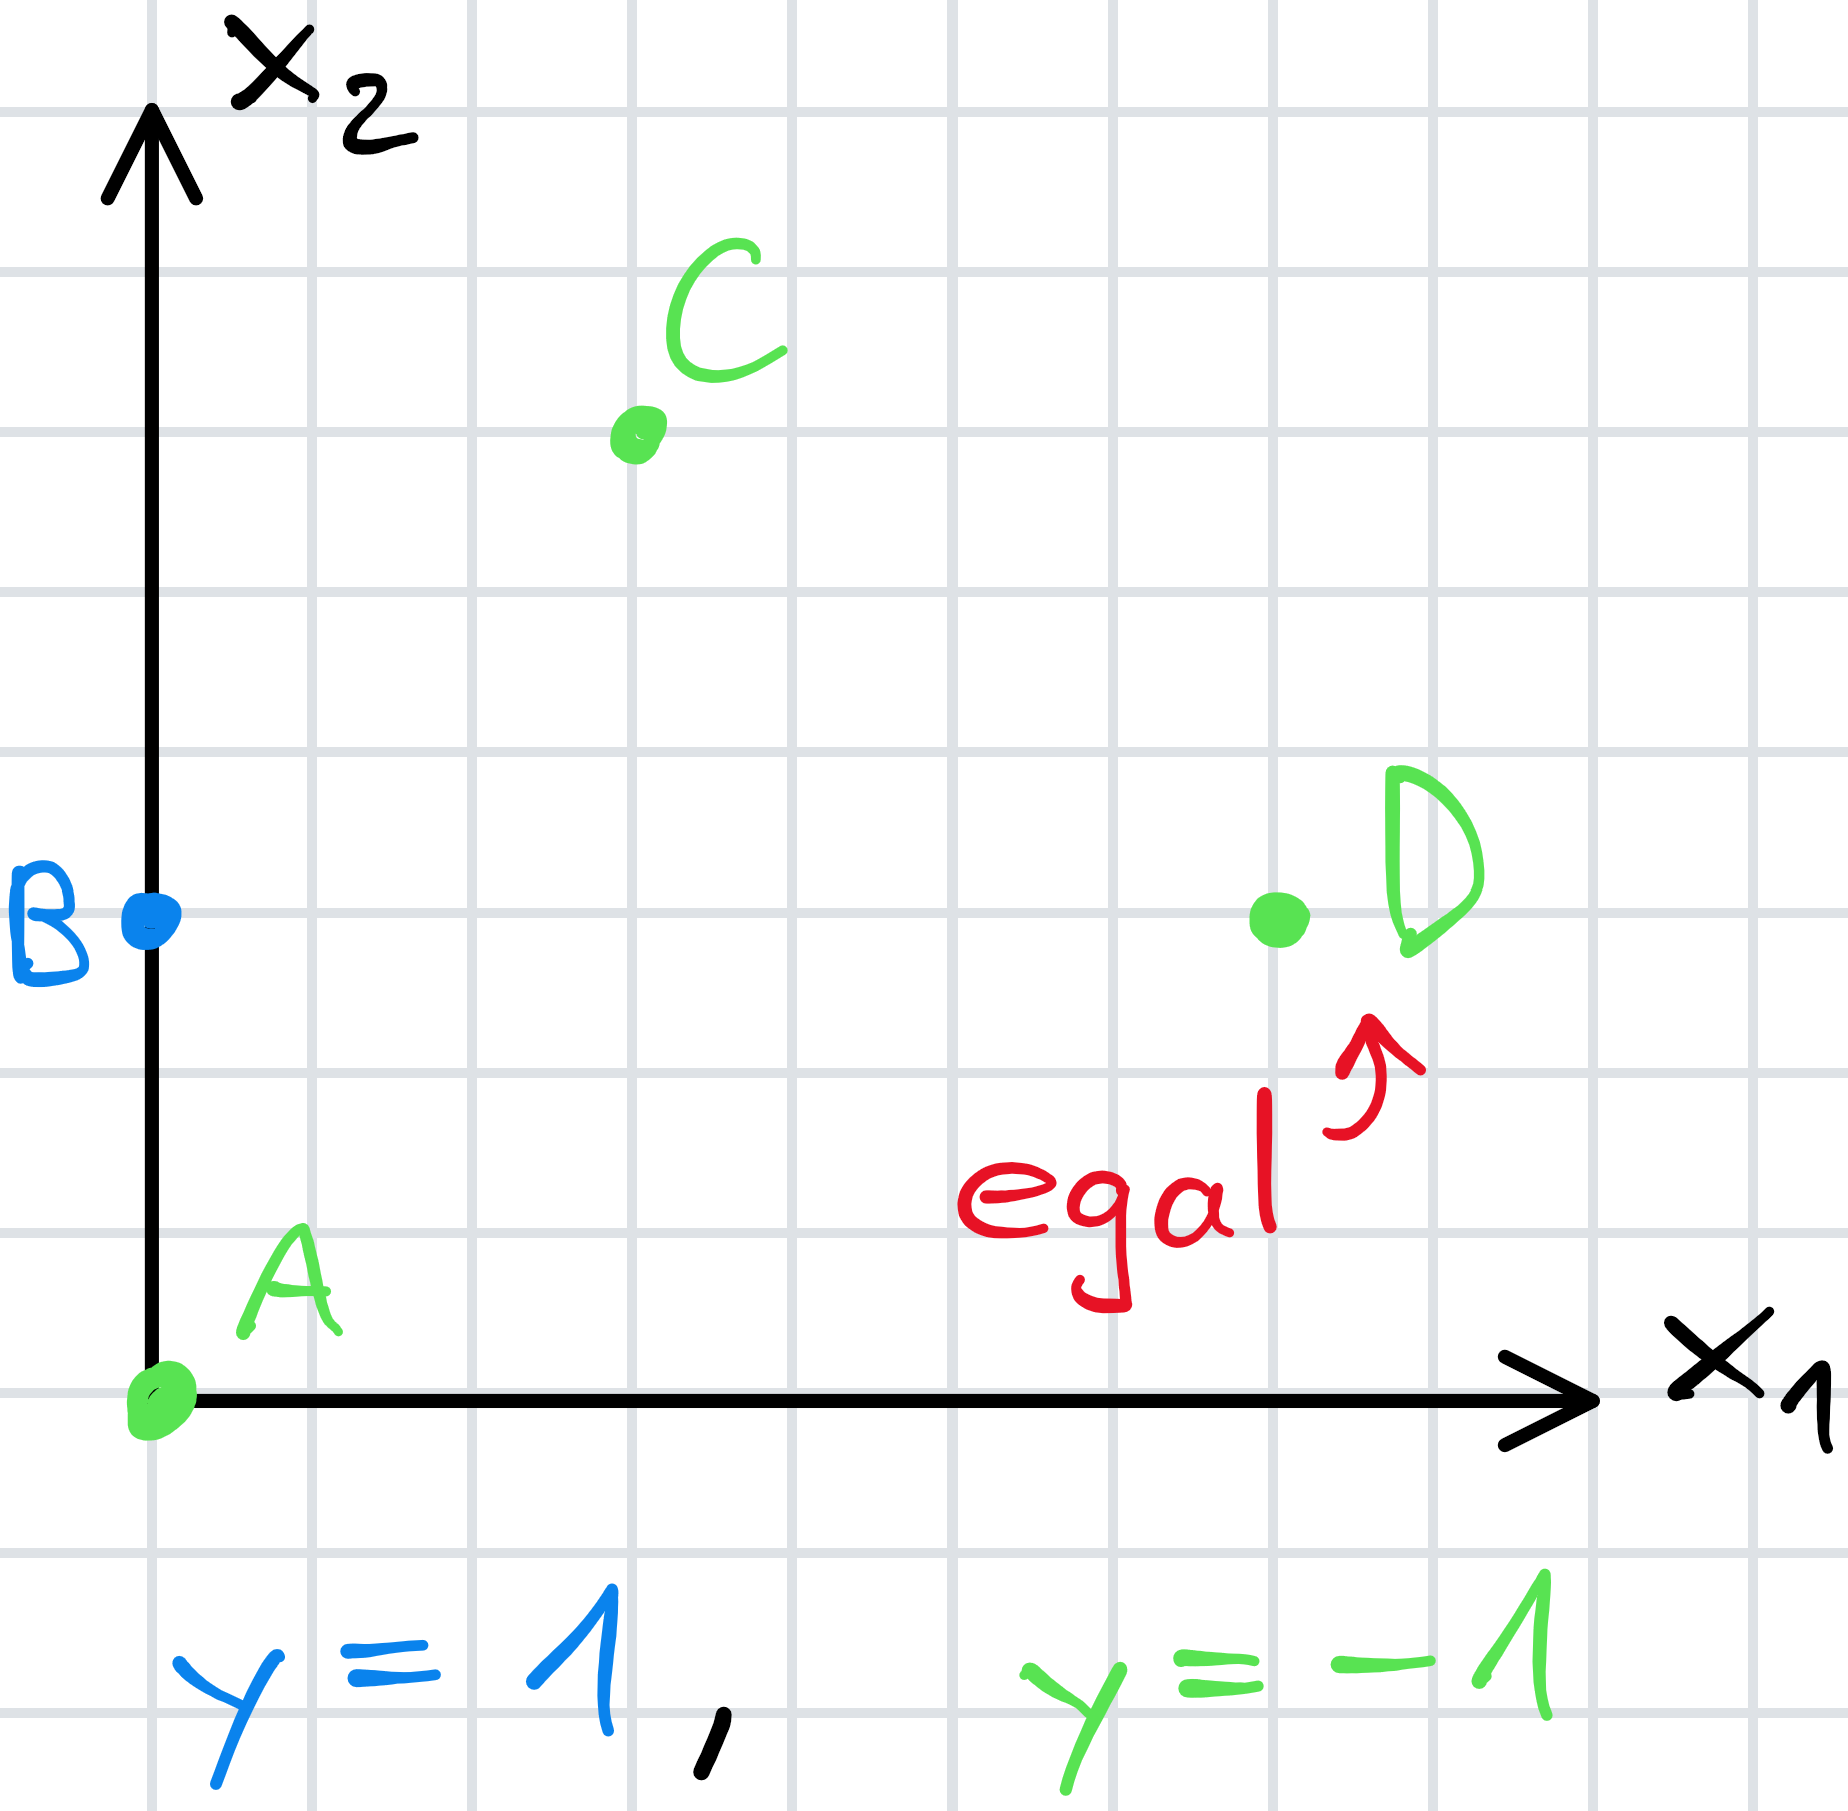
\includegraphics[width=\columnwidth]{images/SVM_2.png}
    \end{minipage}
    
    \item \myul{\textbf{Nebenbedingungen, Es muss gelten:}}
    \begin{itemize}
        \item [\textbf{a:}] $\boxed{\alpha_j\geq0}$
        \item [\textbf{b:}] $\boxed{\sum_{j=1}^N\alpha_j \cdot y_j=0}$\\
        Nach einem $\alpha$ unstellen und anschliessend jenes $\alpha$\\(damit die Nebenbedingung miteinbezogen wird) in der Lagrange-Funktion ersetzen
    \end{itemize}
    \item \myul{\textbf{Kernel-Matrix aufstellen:}}\\
        $\boxed{K\left( \vec{x}^{\text{ $tr$}} ; \vec{x}\right) = \vec{x}^{\text{ $tr$}} \bullet \vec{x}}$\\
        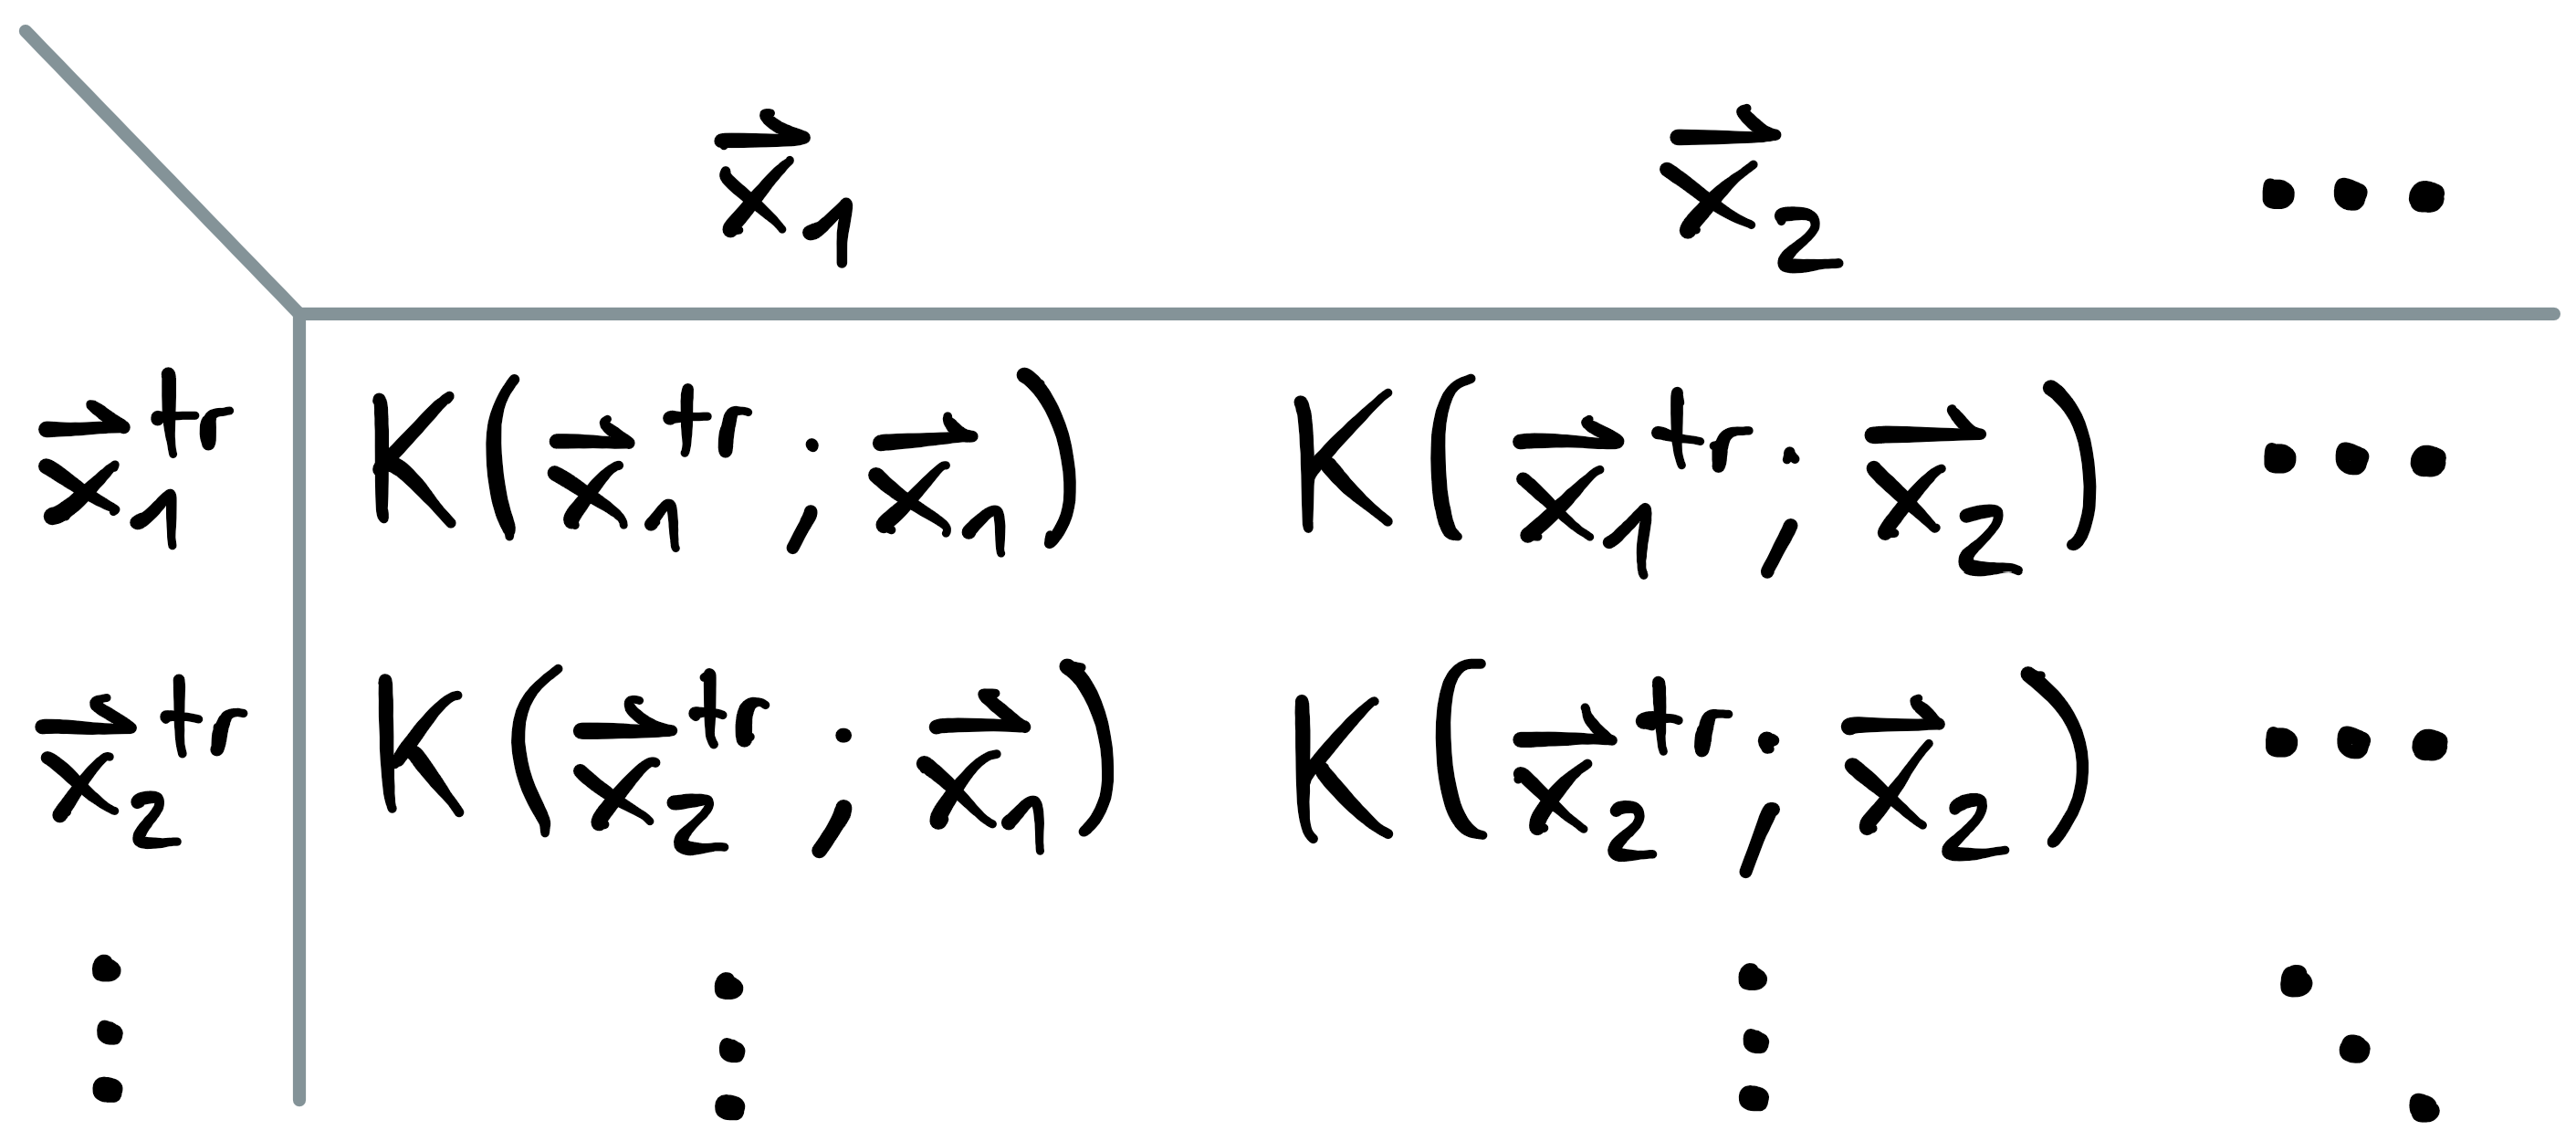
\includegraphics[width=5cm]{images/kernel_matrix.png}
        \begin{itemize}
            \item Einträge sind die Ergebnisse der Skalarprodukte
        \end{itemize}
    \item \myul{\textbf{Lagrange-Funktion aufstellen:}}\\
        $\boxed{L(\vec{\alpha})=\sum_{j=1}^N\alpha_j-\frac{1}{2}\sum_{j,j'=1}^N\alpha_j \cdot \alpha_{j'} \cdot \space y_j \cdot y_{j'} \cdot \space \vec{x}_j^{\text{ $tr$}} \bullet  \vec{x}_{j'}\quad\to\quad\max!}$
        \begin{itemize}
            \item \textbf{2. b} und \textbf{3} brauchen
        \end{itemize}
    \item \myul{\textbf{Alle $\alpha$ finden durch Stationaritätsbedingung}}\\
            $\boxed{\nabla L = \vec{0}}$\\
            $\Rightarrow$ ersetztes $\alpha$ mit gefundenen $\alpha$ berechnen 
    \item \myul{\textbf{$\bm{\vec{w}}$ berechnen:}}\\
        $\boxed{\vec{w}=\sum_{j=1}^N\alpha_jy_j\vec{x}_j}$
    \item \myul{\textbf{Konstante $\mathbf{b}$ berechnen:}}\\
        Datenpunkte mit der Klasse $y = 1$ oder $y = -1$ wählen und einsetzen
        \begin{itemize}
            \item \textbf{Variante 1:} Stützvektor-Datenpunkt mit $y = +1$\\
                $\boxed{\vec{w}^{tr}\cdot\vec{x}_{...} + b = 1} \Leftrightarrow  \boxed{b = 1 -\vec{w}^{tr}\cdot\vec{x}_{...} = ...}$
            \item \textbf{Variante 2:} Stützvektor-Datenpunkt mit $y = -1$\\
                $\boxed{\vec{w}^{tr}\cdot\vec{x}_{...} + b = -1} \Leftrightarrow  \boxed{b = -1 -\vec{w}^{tr}\cdot\vec{x}_{...} = ...}$
        \end{itemize}
\end{enumerate}


\subsection{Nicht linear Trennbare Daten}
Sollte ein Datensatz von nicht linear trennbaren Datenpunkten vorliegen, so muss dieser durch eine Transformation linear trennbar gemacht werden.
Dadurch werden die Punkte oft in höhere Dimensionen gebracht.
Das Finden einer geeigneten Transformation liegt nicht im Ramen dieses Moduls.

Der einzige Unterschied zu der Methode zum linearen trennen von Datenpunkten ist dann, dass stat mit den Datenpunkten $\vec{x}_i$ mit deren durch $\varphi$ transformierten gegenstücken $\vec{\varphi}(\vec{x}_i)$ gerechnet wird.
        \columnbreak
\section{Koordinatensysteme}
\subsection{2D Koordinatensysteme}
Neben den Kartesischen Koordinatensystemen kommen in zweidimensionalen Räumen auch Polare Koordinatensysteme zum Einsatz.
Die beiden Systeme können mit Hilfe der Trigonometrie in einander überführt werden.

\subsubsection{Umrechnung Kartesisch $\leftrightarrow$ Polar}
\begin{minipage}{0.29\linewidth}
    \myul{Polar zu Kartesisch}
    \[
    \begin{pmatrix}
        x \\
        y
    \end{pmatrix}
    =
    \begin{pmatrix}
        r \cdot \cos{\varphi}\\
        r \cdot \sin{\varphi}
    \end{pmatrix}
    \]
\end{minipage}
\hfill
\begin{minipage}{0.29\linewidth}
    \myul{Kartesisch zu Polar}
    \[
    \begin{pmatrix}
        r \\
        \varphi
    \end{pmatrix}
    =
    \begin{pmatrix}
        \sqrt{x^2+y^2}\\
        \tan^{-1}{\frac{y}{x}}
    \end{pmatrix}
    \]
\end{minipage}
\hfill
\begin{minipage}{0.29\linewidth}
    \begin{center}
        \begin{tikzpicture} [scale = 1.5]
            % Kartesische Achsen
            \draw[-{latex}] (0, 0) -- (1, 0) node [below] {$x$} ;
            \draw[-{latex}] (0, 0) -- (0, 1) node [left]  {$y$} ;

            % Punkt p
            \fill (0.5, 0.8) circle (1pt) node [anchor=south west] {$\vec{p}$};

            % Länge r
            \draw (0, 0) -- (0.5, 0.8) node [midway, above left] {$r$};
            % Winkel phi
            \draw [-{latex}] (0.5, 0) arc (0:58:0.5) node [midway, right] {$\varphi$};
        \end{tikzpicture}
    \end{center}
\end{minipage}

Dabei ist zu beachten, dass $\tan^{-1}$ nur werte von $-\frac{\pi}{2}$ bis $\frac{\pi}{2}$ liefert, für $\varphi$ jedoch $\varphi \in [0, \pi]$ gelten soll. 
$\varphi$ wird also, je nach dem in welchem Quadranten sich $\vec{p}$ befindet, nach folgendem Schema berechnet:
\begin{center}
    \begin{tikzpicture}
        % Achsen 
        \draw [-{latex}] (-2, 0) -- (2, 0) node [below] {$x$};
        \draw [-{latex}] (0, -0.8) -- (0, 0.8) node [left] {$y$};
        % Formeln
        \node at ( 1,  0.4) {$       \tan^{-1}\frac{y}{x}$};
        \node at ( 1, -0.4) {$2\pi + \tan^{-1}\frac{y}{x}$};
        \node at (-1, -0.4) {$\pi  + \tan^{-1}\frac{y}{x}$};
        \node at (-1,  0.4) {$\pi  + \tan^{-1}\frac{y}{x}$};
    \end{tikzpicture}
\end{center}

Um eine ganzes Integral vom einen Koordinatensystem ins andere zu überführen, muss zum einen die Funktion $ f(x, y) $ zu $ f(r, \varphi) $ (oder umgekehrt) umgeschrieben, sowie die differentiale angepasst werden.
Hier dafür einige gängige Elemente:

\begin{tabular}{l c c}
                         & \bf{Kartesisch}                   & \bf{Polar}                                                       \\
    \bf{x-Achsenelement} & $\diff x$                         & $\diff x = \cos \varphi \diff r - r \sin \varphi \diff \varphi$  \\
    \bf{y-Achsenelement} & $\diff y$                         & $\diff x = \sin \varphi \diff r + r \cos \varphi \diff \varphi$  \\
    \bf{Linienelement  } & $\diff s^2 = \diff x^2 \diff y^2$ & $\diff s^2 = \diff r^2 + r^2 \diff \varphi^2$                    \\
    \bf{Flächenelement } & $\diff A = \diff x \diff y$       & $\diff A = r \diff r \diff \varphi$                              \\
\end{tabular}


\subsection{3D Koordinatensysteme}
\resizebox{\linewidth}{!}{
    \begin{tabular}{c c c}
        \myul{\textbf{Kartesisch}} & \myul{\textbf{Zylindrisch}} & \myul{\textbf{Sphärisch}} \\
        
        \tdplotsetmaincoords{70}{110}
        \begin{tikzpicture}[baseline=(current bounding box.north), tdplot_main_coords, scale=2]
            % Koordinatensystem
            \draw [-{latex}] (0, 0, 0) -- (1, 0, 0) node [below left] {$x$};
            \draw [-{latex}] (0, 0, 0) -- (0, 1, 0) node [right]      {$y$};
            \draw [-{latex}] (0, 0, 0) -- (0, 0, 1) node [right]      {$z$};
            % Punkt bei (0.75,0.75,0.75)
            \fill (0.75, 0.75, 0.75) circle (1pt) node [above right] {$P(x, y, z)$};
            % Koordinatenkomponenten
            \draw [dashed] (0, 0.75, 0)    -- (0.75, 0.75, 0)    node [midway, below right] {$x$};
            \draw [dashed] (0.75, 0, 0)    -- (0.75, 0.75, 0)    node [midway, below left]  {$y$};
            \draw [dashed] (0.75, 0.75, 0) -- (0.75, 0.75, 0.75) node [midway, right]       {$z$};
        \end{tikzpicture} &

        \tdplotsetmaincoords{70}{110}
        \begin{tikzpicture}[baseline=(current bounding box.north), tdplot_main_coords, scale=2]
            % Koordinatensystem
            \draw [-{latex}] (0, 0, 0) -- (1, 0, 0) node [below left] {$x$};
            \draw [-{latex}] (0, 0, 0) -- (0, 1, 0) node [right]      {$y$};
            \draw [-{latex}] (0, 0, 0) -- (0, 0, 1) node [right]      {$z$};
            % Punkt bei (0.75,0.75,0.75)
            \fill (0.75, 0.75, 0.75) circle (1pt) node [above right] {$P(r_{\rm z}, \varphi, z)$};
            % Koordinatenkomponenten
            \draw [dashed] (0,0,0)         --  (0.75, 0.75, 0)    node [midway, above right, inner sep=0pt] {$r_{\rm z}$};
            \draw [-{latex}]     (0.5,0,0)       arc (0:45:0.5)         node [midway, below]       {$\varphi$};
            \draw [dashed] (0.75, 0.75, 0) --  (0.75, 0.75, 0.75) node [midway, right]       {$z$};
        \end{tikzpicture} &

        \tdplotsetmaincoords{70}{110}
        \begin{tikzpicture}[baseline=(current bounding box.north), tdplot_main_coords, scale=2]
            % Koordinatensystem
            \draw [-{latex}] (0, 0, 0) -- (1, 0, 0) node [below left] {$x$};
            \draw [-{latex}] (0, 0, 0) -- (0, 1, 0) node [right]      {$y$};
            \draw [-{latex}] (0, 0, 0) -- (0, 0, 1) node [right]      {$z$};
            % Punkt bei (0.75,0.75,0.75)
            \fill (0.75, 0.75, 0.75) circle (1pt) node [above right] {$P(r_{\rm s}, \theta, \phi)$};
            % Koordinatenkomponenten
            \draw [dotted] (0,0,0) -- (0.75, 0.75, 0) -- (0.75, 0.75, 0.75);
            \draw [-{latex}]     (0.5,0,0) arc (0:45:0.5)         node [midway, below]       {$\phi$};
            \draw [dashed] (0, 0, 0) --  (0.75, 0.75, 0.75) node [midway, below right] {$r_{\rm s}$};
            \tdplotsetthetaplanecoords {90}
            \tdplotdrawarc [tdplot_rotated_coords, -{latex}] {(0, 0, 0)} {0.5} {0} {45} {anchor=south} {$\theta$}
        \end{tikzpicture} \\

        $ 
        \begin{pmatrix}
            x \\ y \\ z
        \end{pmatrix} 
        =
        \begin{pmatrix}
            r \cos \varphi \\ r \sin \varphi \\ z
        \end{pmatrix}
        =
        \begin{pmatrix}
            r \sin \theta \cos \phi \\ r \sin \theta \sin \phi \\ r \cos \theta
        \end{pmatrix}
        $ &
        $ 
        \begin{pmatrix}
            r_{\rm z} \\ \varphi \\ z
        \end{pmatrix} 
        =
        \begin{pmatrix}
            \sqrt{x^2 + y^2} \\ \tan^{-1}\frac{y}{x} \\ z
        \end{pmatrix}
        =
        \begin{pmatrix}
            r_{\rm s} \sin \theta \\ \phi \\ r_{\rm s} \cos \theta
        \end{pmatrix}
        $ &
        $ 
        \begin{pmatrix}
            r_{\rm s} \\ \theta \\ \phi
        \end{pmatrix} 
        =
        \begin{pmatrix}
            \sqrt{x^2+y^2+z^2} \\ \cos^{-1} \frac{z}{\sqrt{x^2+y^2+z^2}} \\ \sgn(y) \cos^{-1} \frac{x}{\sqrt{x^2+y^2}}
        \end{pmatrix}
        =
        \begin{pmatrix}
            \sqrt{r_{\rm z}^2+z^2} \\ \tan^{-1}\frac{r_{\rm z}}{z} \\ \varphi
        \end{pmatrix}
        $ \\
    \end{tabular}
}
\smallskip
\subsubsection{Umrechnen zwischen Koordinatensystemen}
Beim Umrechnen zwischen den Koordinatensystemen gelten im Grunde genommen die obigen Formeln. 
Dabei muss jedoch in einigen Fällen auf die Wertebereiche von den trigonometrischen Funktionen rücksicht genommen werden.

\myul{\textbf{Zylindrisch $\rightarrow$ Kartesisch:}}\\
\myul{\textbf{Sphärisch $\rightarrow$ Kartesisch:}}\\
Keine weiteren Berücksichtigungen nötig, die Berechnung erfolgt nach der Formel oben.
\medskip

\myul{\textbf{Kartesisch $\rightarrow$ Zylindrisch:}}\\
\begin{minipage}{0.49\linewidth}
    Der Parameter $\phi$ wird analog zum zweidimensionalen Fall, je nach dem in welchem Quadranten sich $P$ befindet, nach dem Schema rechts berechnet.
\end{minipage}
\hfill
\begin{minipage}{0.49\linewidth}
    \begin{center}
        \begin{tikzpicture}
            % Achsen 
            \draw [-{latex}] (-2, 0) -- (2, 0) node [below] {$x$};
            \draw [-{latex}] (0, -0.8) -- (0, 0.8) node [left] {$y$};
            % Formeln
            \node at ( 1,  0.4) {$       \tan^{-1}\frac{y}{x}$};
            \node at ( 1, -0.4) {$2\pi + \tan^{-1}\frac{y}{x}$};
            \node at (-1, -0.4) {$ \pi + \tan^{-1}\frac{y}{x}$};
            \node at (-1,  0.4) {$ \pi + \tan^{-1}\frac{y}{x}$};
        \end{tikzpicture}
    \end{center}
\end{minipage}
\medskip

\myul{\textbf{Sphärisch $\rightarrow$ Zylindrisch:}}\\
\myul{\textbf{Kartesisch $\rightarrow$ Sphärisch:}}\\
Keine weiteren Berücksichtigungen nötig, die Berechnung erfolgt nach der Formel oben.
\medskip

\myul{\textbf{Zylindrisch $\rightarrow$ Sphärisch:}}\\
\begin{minipage}{0.49\linewidth}
    Auch hier macht der $\tan^{-1}$ Probleme, da er Werte von $-\frac{\pi}{2}$ bis $\frac{\pi}{2}$ liefert, für $\theta$ jedoch $\theta \in [0, \pi]$ gelten soll.
    Je nach dem, ob $P$ sich oberhalb oder unterhalb der $xy$-Ebene befindet, wird $\theta$ wie rechts berechnet.
\end{minipage}
\hfill
\begin{minipage}{0.49\linewidth}
    \begin{center}
        \begin{tikzpicture}
            % Achsen 
            \draw [-{latex}] (-2,  0)   -- (2, 0) node [below] {$xy$-Ebene};
            \draw [-{latex}] ( 0, -0.8) -- (0,.9) node [left]  {$z$};
            % Formeln
            \node [fill=white] at (0,  0.4) {$\tan^{-1}\frac{r_{\rm z}}{z}$};
            \node [fill=white] at (0, -0.4) {$\pi + \tan^{-1}\frac{r_{\rm z}}{z}$};
        \end{tikzpicture}
    \end{center}
\end{minipage}


        \columnbreak
\section{Integration}
\subsection{Allgemeines}
Unter bi- oder multivariater Integration versteht man Integrale, welche sich über zwei oder mehr unabhängige Variablen erstrecken.
Sie haben die Form:
\[
    \int\limits_{\Omega} f(\omega) \diff \omega = \iint \cdots \int f(x_1, x_2, \ldots, x_n) \diff x_1 \diff x_2 \cdots \diff x_n
    \quad |\; \Omega \in \rreal^n
\]

\subsection{Normalbereiche}
Unter einem Normalbereich versteht man einen Bereich, welcher in allen Dimensionen so begrenzt ist, 
dass eine Funktion $f(x_1, x_2, \ldots, x_n)$ für jeden Eingangsvektor jeweils nur einen Funktionswert zurückgibt.


\example{Normalbereich in 2D}
% DONE: insert Normalbereich Image
\begin{center}
    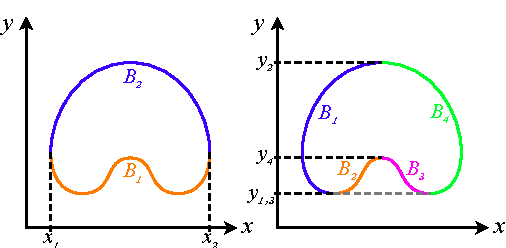
\includegraphics[width=0.8\columnwidth]{images/Normalbereiche_2D.pdf}
\end{center}
% TODO: add caption


\subsection{Satz von Fubini (Satz von Tonelli)}
Der Satz von Fubini besagt, dass die Reihenfolge der Integrationen vertauscht werden kann, sofern die Funktion integrierbar ist.

\[
    \iint\limits_{y_1 x_1}^{\; y_2 x_2} f(x,y)\diff x \diff y = \iint\limits_{x_1 y_1}^{\; x_2 y_2} f(x,y)\diff y \diff x%\iint f(x, y) \diff x \diff y = \int \left\lgroup \int f(x, y) \diff x \right\rgroup \diff y = \int \left\lgroup \int f(x, y) \diff y \right\rgroup \diff x
\]


\subsection{Erster Metrischer Tensor} % TODO: Vereinheitlichung d. Variablen und Funktionen
Der 1. metrische Tensor (oder auch \textbf{erste Fundamentalmatrix}, \textbf{erste Fundamentalform}, \textbf{metrische Grundform})
beschreibt den Zusammenhang zwischen einer Kurve oder Fläche im Parameterraum zum Raum, in dem sie sich befindet (z.B. 2D-Fläche im 3D-Raum).
Er besteht aus den Skalarprodukten der partiellen Ableitungsvektoren nach den Parametern.
\[
    g_{ij} = \frac{\partial \vec{S}}{\partial u_i} \dotp \frac{\partial \vec{S}}{\partial u_j}
\]
Folglich ergibt sich die Matrix: $\begin{pmatrix}
    E & F\\
    F & G
\end{pmatrix} = \begin{pmatrix}
    g_{11} & g_{12}\\
    g_{21} & g_{22}
\end{pmatrix}$

Die Einträge dieser Matrix werden benötigt, um Längen- oder Flächen(elemente) zu berechnen.

% TODO: subsubsection Flächen-, Längen- & Winkelerhaltung (Siehe Moodle Woche 11)

\example{Längenberechnung}
Eine Flächenkurve sei als $\vec{x}(t) = \begin{pmatrix}
    u(t)\\
    v(t)
\end{pmatrix}$ gegeben.
Davon wird das totale Differential gebildet: 
\[
    \dot{\vec{x}} = \vec{x}_u \cdot \dot{u} + \vec{x}_v \cdot \dot{v}
\]
Um die Länge des Vektors (Längenelement) zu erhalten, muss man diesen im ersten Schritt quadrieren:
\[
    (\dot{\vec{x}})^2 = g_{11} \dot{u}^2 + 2 g_{12} \dot{u} \dot{v} + g_{22} \dot{v}^2
\]
Das einzelne Längenelement ist somit:
\[
    \diff s = \sqrt{g_{11} \diff u^2 + 2 g_{12} \diff u \diff v + g_{22} \diff v^2}
\]
Summiert man nun alle $\diff s$ über die Kurve, so ergibt dies das Integral für die gesamte Länge:
\[
    s = \int\limits_{a}^{b} \sqrt{g_{11} \dot{u}^2 + 2 g_{12} \dot{u} \dot{v} + g_{22} \dot{v}^2} \diff t
\]


\example{Flächenberechnung}
Es sei eine parametrisierte Fläche als Funktion $\vec{S}(u,v) = \begin{pmatrix}
    x(u,v)\\
    y(u,v)\\
    z(u,v)
\end{pmatrix}$ gegeben.
Das Flächenelement lässt sich aus einem Parallelogramm der beiden partiellen Ableitungsvektoren bilden, 
was dem Betrag des Kreuzproduktes bzw. der Determinante entspricht:
\[
    \diff S = \sqrt{\abs{\det\abs{g_{ij}}}}\diff u \diff v = \sqrt{g_{11}g_{22} - g_{12}^2} \diff u \diff v = \abs{\frac{\partial \vec{S}}{\partial u} \times \frac{\partial \vec{S}}{\partial v}} \diff u \diff v
\]
Daraus ergibt sich die Fläche über das Doppelintegral:
\[
    S = \iint\limits_{v_1\, u_1}^{v_2\, u_2} \sqrt{g_{11}g_{22} - g_{12}^2} \diff u \diff v
\]


% DONE: Längenintegrale (3D)
% TODO: Längenintegrale (2D)
\subsection{Längenintegrale}
\subsubsection{Längenelemente}\label{section:int_multivar:längenelemente}
$$
 \diff s^2 
    = \underbrace{\diff x^2 + \diff y^2 + \diff z^2}_{\text{Kartesisch}}
    = \underbrace{\diff r^2 + r^2 \diff \varphi^2 + \diff z^2}_{\text{Zylindrisch}}
    = \underbrace{\diff r^2 + r^2 \diff \theta^2 + r^2 \sin^2 \theta \diff \phi^2}_{\text{Sphärisch}}
$$
\subsubsection{Kurvenintegrale 1. Art: Länge einer Funktion}
Die Bestimmung der Länge einer Kurve kann in folgende Schritte unterteilt werden:
\begin{enumerate}
    \item \myul{\textbf{Funktion in die Parameterdarstellung überführen (sofern nicht gegeben):}}
    \item[] Dafür wird einer der Parameter (z.B. $x$ oder $\theta$) $=t$ gesetzt und die anderen Parameter ebenfalls als Funktion von $t$ ausgedrückt.
    \item \myul{\textbf{Integral aufstellen:}}
    \item[] Das Integral in der Form $ \iiint \diff s $ wird mit $\frac{\diff t}{\diff t}$ erweitert.
    \item \myul{\textbf{Das Integral lösen}}
\end{enumerate}

% \subsubsection{Beispiel}
\example{Längenintegral in kartesischen Koordinaten}
Es soll die Länge der Kurve $\vec{v}(t) = \begin{pmatrix}x(t)\\y(t)\\z(t)\end{pmatrix}$ auf dem Interval $[t_1, t_2]$ bestimmt werden.
Dazu werden die oben genannten Schritte abgearbeitet:
\begin{enumerate}
    \item \textbf{Funktion in die Parameterdarstellung überführen}
    \item[] Hier nicht nötig. % evtl. TODO: Beispiel wählen, bei dem das nötig ist.
    \item \textbf{Integral aufstellen} 
    \item[] $ \iiint \diff s = \iiint \sqrt{\diff x^2 + \diff y^2 + \diff z^2} = \int_{t_1}^{t_2} \sqrt{\left(\frac{\diff x}{\diff t}\right)^2 + \left(\frac{\diff y}{\diff t}\right)^2 + \left(\frac{\diff z}{\diff t}\right)^2} \diff t$
    \item Integral lösen
    \item[] $\frac{\diff x}{\diff t}$, $\frac{\diff y}{\diff t}$ und $\frac{\diff z}{\diff t}$ ausrechnen, einsetzen, integrieren.
\end{enumerate}

\subsubsection{Kurvenintegral 2. Art}
Beim Kurvenintegral 2. Art wird nicht die tatsächliche Länge einer Funktion, sondern die Länge deren Projektion auf eine Achse bestimmt.
Dazu wird stat über alle Koordinatenrichtungen nur über eine der Koordinaten integriert.

Es folgen einige Paare von Kurvenintegralen 2. Art entlang einer Kontur $K$ für Funktionen in expliziter Form und in Parameterdarstellung.

\myul{2D, Projektion auf x:}
\[
    \int\limits_{K}f(x)dx = \int_{t_0}^{T}\vec{f}(x(t), y(t)) \cdot x'(t) \cdot dt
\]

\myul{3D, Projektion auf x:}
\[
    \int\limits_{K}f(x, y)dx = \int_{t_0}^{T}\vec{f}(x(t), y(t), z(t)) \cdot x'(t) \cdot dt
\]


% DONE: Flächenintegrale (2D, 3D)
\subsection{(Ober-)Flächenintegrale}
\subsubsection{Flächenelemente}
% TODO: stimmt das?
Das Bestimmen der Flächenelemente ist in drei Dimensionen nicht wie bei den Längen- und Volumenelementen pauschal möglich.
Dies, da jeweils nur über zwei der drei Koordinaten integriert werden muss.
Ein einfaches Verfahren für das Berechnen von Flächeninhalten schafft jedoch abhilfe.
\subsubsection{Flächeninhalt einer Oberfläche}
Für das Berechnen der Oberflächen von Funktionen des Typs $f(a, b)$ in 3D kann die Formel
$$ S = \int\limits_{B} \int\limits_{A} \sqrt{(f_{a})^2 + (f_{b})^2 + 1} \diff a \diff b $$
verwendet werden. Dabei repräsentieren $a$ und $b$ die beiden Koordinatenrichtungen, in denen sich die Fläche erstreckt.
$f_a$ und $f_b$ sind die partiellen Ableitungen der Funktion $f(a, b)$ nach $a$ bzw. $b$.
\medskip

\myul{\bf{Beispiele zur Veranschaulichung:}}\\
Es soll die Oberfläche der Funktion $ f(x, y) $ im Bereich $ x \in [x_1, x_2], y \in [y_1, y-2] $ bestimmt werden.
Das entsprechende integral lautet:
$$ S = \int_{y_1}^{y_2} \int_{x_1}^{x_2} \sqrt{(f_{x})^2 + (f_{y})^2 + 1} \diff x \diff y $$

Wäre die Funktion $f$ stat in kartesischen in polaren oder sphärischen Koordinaten formuliert, ändern sich lediglich die Namen der Variablen. 
Folglich ist das zu einer in sphärischen Koordinaten definierten Fkt. $f(\theta, \phi)$ gehörende Integral
$$ S = \int_{\phi_1}^{\phi_2} \int_{\theta_1}^{\theta_2} \sqrt{(f_{\theta})^2 + (f_{\phi})^2 + 1} \diff \theta \diff \phi $$
sehr leicht aufzustellen.


\subsubsection{Allgemeine Wendelfläche}
Die allgemeine Wendelfläche rotiert und verschiebt eine parametrisierte 3D Kurve $\vec{r}(t) = (x(t), y(t), z(t))\tr$ im Raum.

Parametrisierung bei vertikaler Rotationsachse und vertikaler Verschiebungsrichtung ($z$-Achse):
\[
    \vec{S}(t, \varphi) = \begin{pmatrix}
        \begin{pmatrix}
            \cos(\varphi) & -\sin(\varphi)\\
            \sin(\varphi) & \cos(\varphi)
        \end{pmatrix}
        \cdot \begin{pmatrix}
            x(t)\\
            y(t)
        \end{pmatrix}\\
        z(t) + c \cdot \varphi
    \end{pmatrix}
    \quad (t_1 \leq t \leq t_2, \land \varphi \in \rreal\;, c \equiv const.)
\]

Bei $c = 1$ \textrightarrow\ Voller Meter bei einer Kurve % TODO: Check this



% TODO: Volumenintegrale (3D)
\subsection{Volumenintegrale}
\subsubsection{Volumenelemente}
$$ 
 \diff V 
    = \underbrace{\diff x \diff y \diff z}_{\text{Kartesisch}}
    = \underbrace{r \diff r \diff \varphi \diff z}_{\text{Zylindrisch}}
    = \underbrace{r^2 \sin \theta \diff \theta \diff \phi \diff r}_{\text{Sphärisch}}
$$


% TODO: Andwendungsformeln
% \subsection{Anwendungsformeln}
% TODO: Anwendungsformeln 2D (Doppelintegrale)
% custom big strut for vertical spacing in tables
\subsection{Anwendungsformeln 2D (Doppelintegrale)}
\resizebox{\linewidth}{!}{
    \begin{tabular}{|l|l|l|}
        \hline
        \bf{Allgemein} & \bf{Kartesische Koordinaten} & \bf{Polarkoordinaten} \\
        \hline

        \multicolumn{3}{|l|}{\bf{Flächeninhalt einer ebenen Figur $F$}} \\\hline
        \bigstrut[tb]$\mathstrut A = \iint\limits_{F} \diff F $ & 
        $ = \int\limits_{X}\int\limits_{Y} \diff y \diff x $ &
        $ = \int\limits_{\Phi}\int\limits_{R} r \diff r \diff \varphi $ \\\hline

        \multicolumn{3}{|l|}{\bf{Oberfläche einer Ebene in drei Dimensionen}} \\\hline
        % TODO: Evtl. umschreiben, dass man es besser versteht...
        \bigstrut[tb]$ S = \iint\limits_{A} \frac{1}{\cos \gamma} \diff A $ & 
        $ = \int\limits_{X}\int\limits_{Y} \sqrt{1 + \left(\frac{\partial z}{\partial x}\right)^2 + \left(\frac{\partial z}{\partial y}\right)^2} \diff y \diff x $ &
        $ = \int\limits_{\Phi}\int\limits_{R} \sqrt{r^2 + r^2\left(\frac{\partial z}{\partial r}\right)^2 + \left(\frac{\partial z}{\partial \varphi}\right)^2} \diff r \diff \varphi $ \\\hline
        
        \multicolumn{3}{|l|}{\bf{Volumen eines Zylinders}} \\\hline
        \bigstrut[tb]$ V = \iint\limits_{A} z \diff A $ & 
        $ = \int\limits_{X}\int\limits_{Y} z \diff y \diff x $ &
        $ = \int\limits_{\Phi}\int\limits_{R} z r \diff r \diff \varphi $ \\\hline

        \multicolumn{3}{|l|}{\bf{Trägheitsmoment einer ebenen Figur $F$, bezogen auf die x-Achse}} \\\hline
        \bigstrut[tb]$ I_x = \iint\limits_{F} y^2 \diff F $ & 
        $ = \int\limits_{X}\int\limits_{Y} (y^2) \diff y \diff x $ &
        $ = \int\limits_{\Phi}\int\limits_{R} (r^2 \sin^2\varphi) r \diff r \diff \varphi $ \\\hline

        \multicolumn{3}{|l|}{\bf{Trägheitsmoment einer ebenen Figur $F$, bezogen auf den Pol $(0, 0)$}} \\\hline
        \bigstrut[tb]$ I_x = \iint\limits_{F} r^2 \diff F $ & 
        $ = \int\limits_{X}\int\limits_{Y} (x^2 + y^2) \diff y \diff x $ &
        $ = \int\limits_{\Phi}\int\limits_{R} (r^2) r \diff r \diff \varphi $ \\\hline

        \multicolumn{3}{|l|}{\bf{Masse einer ebenen Figur $F$ mit Dichtefunktion $\varrho$}} \\\hline
        \bigstrut[tb]$ m = \iint\limits_{F} \varrho \diff F $ & 
        $ = \int\limits_{X}\int\limits_{Y} \varrho (x, y) \diff y \diff x $ &
        $ = \int\limits_{\Phi}\int\limits_{R} \varrho (r, \varphi) r \diff r \diff \varphi $ \\\hline

        \multicolumn{3}{|l|}{\bf{Koordinaten des Schwerpunkts $S$ einer homogenen, ebenen Figur $F$}} \\\hline
        \bigstrut[tb]$ x_{S} = \frac{\strut \iint\limits_{F} x \diff F}{A} $ & 
        $ = \frac{\int\limits_{X}\int\limits_{Y} x \diff y \diff x}{\int\limits_{X}\int\limits_{Y} \diff y \diff x} $ &
        $ = \frac{\int\limits_{\Phi}\int\limits_{R} r^2 \cos \varphi \diff r \diff \varphi}{\int\limits_{\Phi}\int\limits_{R} r \diff r \diff \varphi} $ \\
        \bigstrut[tb]$ y_{S} = \frac{\iint\limits_{F} y \diff F}{A} $ & 
        $ = \frac{\int\limits_{X}\int\limits_{Y} y \diff y \diff x}{\int\limits_{X}\int\limits_{Y} \diff y \diff x} $ &
        $ = \frac{\int\limits_{\Phi}\int\limits_{R} r^2 \sin \varphi \diff r \diff \varphi}{\int\limits_{\Phi}\int\limits_{R} r \diff r \diff \varphi} $ \\\hline
    \end{tabular}
}

\smallskip
Hinweis: Damit die Flächenelemente leichter erkennbar und die Formeln entsprechend besser nachvollziebar sind, wurden sie teilweise nicht vollständig vereinfacht.


% TODO: Anwendungsformeln 3D (Dreifachintegrale)
\subsection{Anwendungsformeln 3D (Dreifachintegrale)}
\resizebox{\linewidth}{!}{
    \begin{tabular}{|l|l|l|l|}  
        \hline
        \bf{Allgemein} & \bf{Kartesische Koordinaten} & \bf{Zylinderkoordinaten} & \bf{Kugelkoordinaten} \\
        \hline
        \multicolumn{4}{|l|}{\bf{Volumen eines Körpers $K$}} \\
        \hline
        \bigstrut[tb]$ V = \iiint\limits_{K} \diff V $ & 
        $ = \iiint \diff x \diff y \diff z $ &
        $ = \iiint r \diff r \diff \phi \diff z $ &
        $ = \iiint r^2 \sin \theta \diff \theta \diff \phi \diff r $ \\
        \hline

        \multicolumn{4}{|l|}{\bf{Trägheitsmoment eines Körpers $K$, bezogen auf die Z-Achse}} \\
        \hline
        \bigstrut[tb]$ I_z = \iiint\limits_{K} r^2 \diff V $ & 
        $ = \iiint (x^2 + y^2) \diff x \diff y \diff z $ &
        $ = \iiint (r^2) r \diff r \diff \phi \diff z $ &
        $ = \iiint (r^2 \sin^2 \theta) r^2 sin \theta \diff \theta \diff \phi \diff r $ \\
        \hline

        \multicolumn{4}{|l|}{\bf{Masse eines Körpers $K$ mit der Dichtefunktion $\varrho$}} \\
        \hline
        \bigstrut[tb]$ M = \iiint\limits_{K} \varrho \diff V $ & 
        $ = \iiint \varrho (x, y, z) \diff x \diff y \diff z $ &
        $ = \iiint \varrho (r, \phi, z) r \diff r \diff \phi \diff z $ &
        $ = \iiint \varrho (r, \theta, \phi) r^2 sin \theta \diff \theta \diff \phi \diff r $ \\
        \hline

        \multicolumn{4}{|l|}{\bf{Koordinaten des Schwerpunktes $S$ eines homogenen Körpers $K$}} \\
        \hline
        $ x_{S} = \frac{\strut \iiint\limits_{K} x \diff V}{V} $ & 
        $ = \frac{\iiint (x) \diff x \diff y \diff z}{V} $ &
        $ = \frac{\iiint (r \cos \phi) r \diff r \diff \phi \diff z}{V} $ &
        $ = \frac{\iiint (r \sin \theta \cos \phi) r^2 sin \theta \diff \theta \diff \phi \diff r}{V} $ \\

        \bigstrut[tb]$ y_{S} = \frac{\iiint\limits_{K} y \diff V}{V} $ & 
        $ = \frac{\iiint (y) \diff x \diff y \diff z}{V} $ &
        $ = \frac{\iiint (r \sin \phi) r \diff r \diff \phi \diff z}{V} $ &
        $ = \frac{\iiint (r \sin \theta \sin \phi) r^2 sin \theta \diff \theta \diff \phi \diff r}{V} $ \\

        \bigstrut[tb]$ z_{S} = \frac{\iiint\limits_{K} z \diff V}{V} $ & 
        $ = \frac{\iiint (z) \diff x \diff y \diff z}{V} $ &
        $ = \frac{\iiint (z) r \diff r \diff \phi \diff z}{V} $ &
        $ = \frac{\iiint (r \cos \theta) r^2 sin \theta \diff \theta \diff \phi \diff r}{V} $ \\
        \hline
    \end{tabular}
}

\smallskip
Hinweis: Damit die Volumenelemente leichter erkennbar und die Formeln entsprechend besser nachvollziebar sind, wurden sie teilweise nicht vollständig vereinfacht.


% \subsection{Umrechnungen}
% \subsubsection{Kartesische Koordinaten $\leftrightarrow$ Polarkoordinaten}

% \subsection{Anwendungsformeln}
% \resizebox{\linewidth}{!}{
%     \begin{tabular}{|l|l|l|}
%         \hline
%         \bf{Allgemein} & \bf{Kartesische Koordinaten} & \bf{Polarkoordinaten} \\
%         \hline

%         \multicolumn{3}{|l|}{\bf{Flächeninhalt einer ebenen Figur $F$}} \\\hline
%         $ A = \iint\limits_{F} \diff a $ & 
%         $ = \int\limits_{X}\int\limits_{Y} \diff y \diff x $ &
%         $ = \int\limits_{\Phi}\int\limits_{R} r \diff r \diff \varphi $ \\\hline

%         \multicolumn{3}{|l|}{\bf{Oberfläche einer Ebene in drei Dimensionen}} \\\hline
%         % TODO: Evtl. umschreiben, dass man es besser versteht...
%         $ S = \iint\limits_{A} \frac{1}{\cos \gamma} \diff a $ & 
%         $ = \int\limits_{X}\int\limits_{Y} \sqrt{1 + \left(\frac{\partial z}{\partial x}\right)^2 + \left(\frac{\partial z}{\partial y}\right)^2} \diff y \diff x $ &
%         $ = \int\limits_{\Phi}\int\limits_{R} \sqrt{r^2 + r^2\left(\frac{\partial z}{\partial r}\right)^2 + \left(\frac{\partial z}{\partial \varphi}\right)^2} \diff r \diff \varphi $ \\\hline
        
%         \multicolumn{3}{|l|}{\bf{Volumen eines Zylinders}} \\\hline
%         $ V = \iint\limits_{A} z \diff a $ & 
%         $ = \int\limits_{X}\int\limits_{Y} z \diff y \diff x $ &
%         $ = \int\limits_{\Phi}\int\limits_{R} z r \diff r \diff \varphi $ \\\hline

%         \multicolumn{3}{|l|}{\bf{Trägheitsmoment einer ebenen Figur $F$, bezogen auf die x-Achse}} \\\hline
%         $ I_x = \iint\limits_{F} y^2 \diff a $ & 
%         $ = \int\limits_{X}\int\limits_{Y} (y^2) \diff y \diff x $ &
%         $ = \int\limits_{\Phi}\int\limits_{R} (r^2 \sin^2\varphi) r \diff r \diff \varphi $ \\\hline

%         \multicolumn{3}{|l|}{\bf{Trägheitsmoment einer ebenen Figur $F$, bezogen auf den Pol $(0, 0)$}} \\\hline
%         $ I_x = \iint\limits_{F} r^2 \diff a $ & 
%         $ = \int\limits_{X}\int\limits_{Y} (x^2 + y^2) \diff y \diff x $ &
%         $ = \int\limits_{\Phi}\int\limits_{R} (r^2) r \diff r \diff \varphi $ \\\hline

%         \multicolumn{3}{|l|}{\bf{Masse einer ebenen Figur $F$ mit Dichtefunktion $\varrho$}} \\\hline
%         $ m = \iint\limits_{F} \varrho \diff a $ & 
%         $ = \int\limits_{X}\int\limits_{Y} \varrho (x, y) \diff y \diff x $ &
%         $ = \int\limits_{\Phi}\int\limits_{R} \varrho (r, \varphi) r \diff r \diff \varphi $ \\\hline

%         \multicolumn{3}{|l|}{\bf{Koordinaten des Schwerpunkts $S$ einer homogenen, ebenen Figur $F$}} \\\hline
%         $ x_{S} = \frac{\iint\limits_{F} x \diff a}{A} $ & 
%         $ = \frac{\int\limits_{X}\int\limits_{Y} x \diff y \diff x}{\int\limits_{X}\int\limits_{Y} \diff y \diff x} $ &
%         $ = \frac{\int\limits_{\Phi}\int\limits_{R} r^2 \cos \varphi \diff r \diff \varphi}{\int\limits_{\Phi}\int\limits_{R} r \diff r \diff \varphi} $ \\
%         $ y_{S} = \frac{\iint\limits_{F} y \diff a}{A} $ & 
%         $ = \frac{\int\limits_{X}\int\limits_{Y} y \diff y \diff x}{\int\limits_{X}\int\limits_{Y} \diff y \diff x} $ &
%         $ = \frac{\int\limits_{\Phi}\int\limits_{R} r^2 \sin \varphi \diff r \diff \varphi}{\int\limits_{\Phi}\int\limits_{R} r \diff r \diff \varphi} $ \\\hline
%     \end{tabular}
% }

% \resizebox{\linewidth}{!}{
%     \begin{tabular}{|l|l|l|l|}  
%         \hline
%         \bf{Allgemein} & \bf{Kartesische Koordinaten} & \bf{Zylinderkoordinaten} & \bf{Kugelkoordinaten} \\
%         \hline
%         \multicolumn{4}{|l|}{\bf{Volumen eines Körpers $K$}} \\
%         \hline
%         $ V = \iiint\limits_{K} \diff V $ & 
%         $ = \iiint \diff x \diff y \diff z $ &
%         $ = \iiint r \diff r \diff \phi \diff z $ &
%         $ = \iiint r^2 \sin \theta \diff \theta \diff \phi \diff r $ \\
%         \hline

%         \multicolumn{4}{|l|}{\bf{Trägheitsmoment eines Körpers $K$, bezogen auf die Z-Achse}} \\
%         \hline
%         $ I_z = \iiint\limits_{K} r^2 \diff V $ & 
%         $ = \iiint (x^2 + y^2) \diff x \diff y \diff z $ &
%         $ = \iiint (r^2) r \diff r \diff \phi \diff z $ &
%         $ = \iiint (r^2 \sin^2 \theta) r^2 sin \theta \diff \theta \diff \phi \diff r $ \\
%         \hline

%         \multicolumn{4}{|l|}{\bf{Masse eines Körpers $K$ mit der Dichtefunktion $\varrho$}} \\
%         \hline
%         $ M = \iiint\limits_{K} \varrho \diff V $ & 
%         $ = \iiint \varrho (x, y, z) \diff x \diff y \diff z $ &
%         $ = \iiint \varrho (r, \phi, z) r \diff r \diff \phi \diff z $ &
%         $ = \iiint \varrho (r, \theta, \phi) r^2 sin \theta \diff \theta \diff \phi \diff r $ \\
%         \hline

%         \multicolumn{4}{|l|}{\bf{Koordinaten des Schwerpunktes $S$ eines homogenen Körpers $K$}} \\
%         \hline
%         $ x_{S} = \frac{\iiint\limits_{K} x \diff V}{V} $ & 
%         $ = \frac{\iiint (x) \diff x \diff y \diff z}{V} $ &
%         $ = \frac{\iiint (r \cos \phi) r \diff r \diff \phi \diff z}{V} $ &
%         $ = \frac{\iiint (r \sin \theta \cos \phi) r^2 sin \theta \diff \theta \diff \phi \diff r}{V} $ \\

%         $ y_{S} = \frac{\iiint\limits_{K} y \diff V}{V} $ & 
%         $ = \frac{\iiint (y) \diff x \diff y \diff z}{V} $ &
%         $ = \frac{\iiint (r \sin \phi) r \diff r \diff \phi \diff z}{V} $ &
%         $ = \frac{\iiint (r \sin \theta \sin \phi) r^2 sin \theta \diff \theta \diff \phi \diff r}{V} $ \\

%         $ z_{S} = \frac{\iiint\limits_{K} z \diff V}{V} $ & 
%         $ = \frac{\iiint (z) \diff x \diff y \diff z}{V} $ &
%         $ = \frac{\iiint (z) r \diff r \diff \phi \diff z}{V} $ &
%         $ = \frac{\iiint (r \cos \theta) r^2 sin \theta \diff \theta \diff \phi \diff r}{V} $ \\
%         \hline
%     \end{tabular}
% }



% \section{Koordinatensysteme}
% \subsection{2D Koordinatensysteme}
% Neben den Kartesischen Koordinatensystemen kommen in zweidimensionalen Räumen auch Polare Koordinatensysteme zum Einsatz.
% Die beiden Systeme können mit Hilfe der Trigonometrie in einander überführt werden.

% \subsubsection{Umrechnung Kartesisch $\leftrightarrow$ Polar}
% \begin{minipage}{0.29\linewidth}
%     \myul{Polar zu Kartesisch}
%     \[
%     \begin{pmatrix}
%         x \\
%         y
%     \end{pmatrix}
%     =
%     \begin{pmatrix}
%         r \cdot \cos{\varphi}\\
%         r \cdot \sin{\varphi}
%     \end{pmatrix}
%     \]
% \end{minipage}
% \hfill
% \begin{minipage}{0.29\linewidth}
%     \myul{Kartesisch zu Polar}
%     \[
%     \begin{pmatrix}
%         r \\
%         \varphi
%     \end{pmatrix}
%     =
%     \begin{pmatrix}
%         \sqrt{x^2+y^2}\\
%         \tan^{-1}{\frac{y}{x}}
%     \end{pmatrix}
%     \]
% \end{minipage}
% \hfill
% \begin{minipage}{0.29\linewidth}
%     \begin{center}
%         \begin{tikzpicture} [scale = 1.5]
%             % Kartesische Achsen
%             \draw[-{latex}] (0, 0) -- (1, 0) node [below] {$x$} ;
%             \draw[-{latex}] (0, 0) -- (0, 1) node [left]  {$y$} ;

%             % Punkt p
%             \fill (0.5, 0.8) circle (1pt) node [anchor=south west] {$\vec{p}$};

%             % Länge r
%             \draw (0, 0) -- (0.5, 0.8) node [midway, above left] {$r$};
%             % Winkel phi
%             \draw [-{latex}] (0.5, 0) arc (0:58:0.5) node [midway, right] {$\varphi$};
%         \end{tikzpicture}
%     \end{center}
% \end{minipage}

% Dabei ist zu beachten, dass $\tan^{-1}$ nur werte von $-\frac{\pi}{2}$ bis $\frac{\pi}{2}$ liefert, für $\varphi$ jedoch $\varphi \in [0, \pi]$ gelten soll. 
% $\varphi$ wird also, je nach dem in welchem Quadranten sich $\vec{p}$ befindet, nach folgendem Schema berechnet:
% \begin{center}
%     \begin{tikzpicture}
%         % Achsen 
%         \draw [-{latex}] (-2, 0) -- (2, 0) node [below] {$x$};
%         \draw [-{latex}] (0, -0.8) -- (0, 0.8) node [left] {$y$};
%         % Formeln
%         \node at ( 1,  0.4) {$       \tan^{-1}\frac{y}{x}$};
%         \node at ( 1, -0.4) {$2\pi + \tan^{-1}\frac{y}{x}$};
%         \node at (-1, -0.4) {$\pi  + \tan^{-1}\frac{y}{x}$};
%         \node at (-1,  0.4) {$\pi  + \tan^{-1}\frac{y}{x}$};
%     \end{tikzpicture}
% \end{center}

% Um eine ganzes Integral vom einen Koordinatensystem ins andere zu überführen, muss zum einen die Funktion $ f(x, y) $ zu $ f(r, \varphi) $ (oder umgekehrt) umgeschrieben, sowie die differentiale angepasst werden.
% Hier dafür einige gängige Elemente:

% \begin{tabular}{l c c}
%                          & \bf{Kartesisch}                   & \bf{Polar}                                                       \\
%     \bf{x-Achsenelement} & $\diff x$                         & $\diff x = \cos \varphi \diff r - r \sin \varphi \diff \varphi$  \\
%     \bf{y-Achsenelement} & $\diff y$                         & $\diff x = \sin \varphi \diff r + r \cos \varphi \diff \varphi$  \\
%     \bf{Linienelement  } & $\diff s^2 = \diff x^2 \diff y^2$ & $\diff s^2 = \diff r^2 + r^2 \diff \varphi^2$                    \\
%     \bf{Flächenelement } & $\diff A = \diff x \diff y$       & $\diff A = r \diff r \diff \varphi$                              \\
% \end{tabular}

% % \subsection{2D Transformation Polar zu Kartesisch}
% % TODO: Das isch ja ds gliiche wie obe beschribe, oder?
% %       Wänn da no meh ane sött wüsstich nöd was... -Flurin
% % T $=$ Transformation
% % \[
% %     \text{Polar } (r,\varphi) \xrightarrow{T} (x,y) \text{ Kartesisch}
% % \]

% % \[
% % \begin{pmatrix}
% %     x=r\cdot\cos(\varphi) \text{ } \cor{\mathbb{R}} \\
% %     y=r\cdot\sin(\varphi) \text{ } \cor{\mathbb{R}} 
% % \end{pmatrix}
% % \text{2D}
% % \]

% % Die Funktionen für $x$ und $y$ sind skalare Funktion.

% %     \begin{ctabular}{ll}
% %         $x=x(r;\varphi)$ & $ y=y(r;\varphi)$
% %     \end{ctabular}


% \subsection{3D Koordinatensysteme}
% \resizebox{\linewidth}{!}{
%     \begin{tabular}{c c c}
%         \myul{\textbf{Kartesisch}} & \myul{\textbf{Zylindrisch}} & \myul{\textbf{Sphärisch}} \\
        
%         \tdplotsetmaincoords{70}{110}
%         \begin{tikzpicture}[baseline=(current bounding box.north), tdplot_main_coords, scale=2]
%             % Koordinatensystem
%             \draw [-{latex}] (0, 0, 0) -- (1, 0, 0) node [below left] {$x$};
%             \draw [-{latex}] (0, 0, 0) -- (0, 1, 0) node [right]      {$y$};
%             \draw [-{latex}] (0, 0, 0) -- (0, 0, 1) node [right]      {$z$};
%             % Punkt bei (0.75,0.75,0.75)
%             \fill (0.75, 0.75, 0.75) circle (1pt) node [above right] {$P(x, y, z)$};
%             % Koordinatenkomponenten
%             \draw [dashed] (0, 0.75, 0)    -- (0.75, 0.75, 0)    node [midway, below right] {$x$};
%             \draw [dashed] (0.75, 0, 0)    -- (0.75, 0.75, 0)    node [midway, below left]  {$y$};
%             \draw [dashed] (0.75, 0.75, 0) -- (0.75, 0.75, 0.75) node [midway, right]       {$z$};
%         \end{tikzpicture} &

%         \tdplotsetmaincoords{70}{110}
%         \begin{tikzpicture}[baseline=(current bounding box.north), tdplot_main_coords, scale=2]
%             % Koordinatensystem
%             \draw [-{latex}] (0, 0, 0) -- (1, 0, 0) node [below left] {$x$};
%             \draw [-{latex}] (0, 0, 0) -- (0, 1, 0) node [right]      {$y$};
%             \draw [-{latex}] (0, 0, 0) -- (0, 0, 1) node [right]      {$z$};
%             % Punkt bei (0.75,0.75,0.75)
%             \fill (0.75, 0.75, 0.75) circle (1pt) node [above right] {$P(r_{\rm z}, \varphi, z)$};
%             % Koordinatenkomponenten
%             \draw [dashed] (0,0,0)         --  (0.75, 0.75, 0)    node [midway, above right, inner sep=0pt] {$r_{\rm z}$};
%             \draw [-{latex}]     (0.5,0,0)       arc (0:45:0.5)         node [midway, below]       {$\varphi$};
%             \draw [dashed] (0.75, 0.75, 0) --  (0.75, 0.75, 0.75) node [midway, right]       {$z$};
%         \end{tikzpicture} &

%         \tdplotsetmaincoords{70}{110}
%         \begin{tikzpicture}[baseline=(current bounding box.north), tdplot_main_coords, scale=2]
%             % Koordinatensystem
%             \draw [-{latex}] (0, 0, 0) -- (1, 0, 0) node [below left] {$x$};
%             \draw [-{latex}] (0, 0, 0) -- (0, 1, 0) node [right]      {$y$};
%             \draw [-{latex}] (0, 0, 0) -- (0, 0, 1) node [right]      {$z$};
%             % Punkt bei (0.75,0.75,0.75)
%             \fill (0.75, 0.75, 0.75) circle (1pt) node [above right] {$P(r_{\rm s}, \theta, \phi)$};
%             % Koordinatenkomponenten
%             \draw [dotted] (0,0,0) -- (0.75, 0.75, 0) -- (0.75, 0.75, 0.75);
%             \draw [-{latex}]     (0.5,0,0) arc (0:45:0.5)         node [midway, below]       {$\phi$};
%             \draw [dashed] (0, 0, 0) --  (0.75, 0.75, 0.75) node [midway, below right] {$r_{\rm s}$};
%             \tdplotsetthetaplanecoords {90}
%             \tdplotdrawarc [tdplot_rotated_coords, -{latex}] {(0, 0, 0)} {0.5} {0} {45} {anchor=south} {$\theta$}
%         \end{tikzpicture} \\

%         $ 
%         \begin{pmatrix}
%             x \\ y \\ z
%         \end{pmatrix} 
%         =
%         \begin{pmatrix}
%             r \cos \varphi \\ r \sin \varphi \\ z
%         \end{pmatrix}
%         =
%         \begin{pmatrix}
%             r \sin \theta \cos \phi \\ r \sin \theta \sin \phi \\ r \cos \theta
%         \end{pmatrix}
%         $ &
%         $ 
%         \begin{pmatrix}
%             r_{\rm z} \\ \varphi \\ z
%         \end{pmatrix} 
%         =
%         \begin{pmatrix}
%             \sqrt{x^2 + y^2} \\ \tan^{-1}\frac{y}{x} \\ z
%         \end{pmatrix}
%         =
%         \begin{pmatrix}
%             r_{\rm s} \sin \theta \\ \phi \\ r_{\rm s} \cos \theta
%         \end{pmatrix}
%         $ &
%         $ 
%         \begin{pmatrix}
%             r_{\rm s} \\ \theta \\ \phi
%         \end{pmatrix} 
%         =
%         \begin{pmatrix}
%             \sqrt{x^2+y^2+z^2} \\ \cos^{-1} \frac{z}{\sqrt{x^2+y^2+z^2}} \\ \sgn(y) \cos^{-1} \frac{x}{\sqrt{x^2+y^2}}
%         \end{pmatrix}
%         =
%         \begin{pmatrix}
%             \sqrt{r_{\rm z}^2+z^2} \\ \tan^{-1}\frac{r_{\rm z}}{z} \\ \varphi
%         \end{pmatrix}
%         $ \\
%     \end{tabular}
% }
% \smallskip
% \subsubsection{Umrechnen zwischen Koordinatensystemen}
% Beim Umrechnen zwischen den Koordinatensystemen gelten im Grunde genommen die obigen Formeln. 
% Dabei muss jedoch in einigen Fällen auf die Wertebereiche von den trigonometrischen Funktionen rücksicht genommen werden.

% \myul{\textbf{Zylindrisch $\rightarrow$ Kartesisch:}}\\
% \myul{\textbf{Sphärisch $\rightarrow$ Kartesisch:}}\\
% Keine weiteren Berücksichtigungen nötig, die Berechnung erfolgt nach der Formel oben.
% \medskip

% \myul{\textbf{Kartesisch $\rightarrow$ Zylindrisch:}}\\
% \begin{minipage}{0.49\linewidth}
%     Der Parameter $\phi$ wird analog zum zweidimensionalen Fall, je nach dem in welchem Quadranten sich $P$ befindet, nach dem Schema rechts berechnet.
% \end{minipage}
% \hfill
% \begin{minipage}{0.49\linewidth}
%     \begin{center}
%         \begin{tikzpicture}
%             % Achsen 
%             \draw [-{latex}] (-2, 0) -- (2, 0) node [below] {$x$};
%             \draw [-{latex}] (0, -0.8) -- (0, 0.8) node [left] {$y$};
%             % Formeln
%             \node at ( 1,  0.4) {$       \tan^{-1}\frac{y}{x}$};
%             \node at ( 1, -0.4) {$2\pi + \tan^{-1}\frac{y}{x}$};
%             \node at (-1, -0.4) {$ \pi + \tan^{-1}\frac{y}{x}$};
%             \node at (-1,  0.4) {$ \pi + \tan^{-1}\frac{y}{x}$};
%         \end{tikzpicture}
%     \end{center}
% \end{minipage}
% \medskip

% \myul{\textbf{Sphärisch $\rightarrow$ Zylindrisch:}}\\
% \myul{\textbf{Kartesisch $\rightarrow$ Sphärisch:}}\\
% Keine weiteren Berücksichtigungen nötig, die Berechnung erfolgt nach der Formel oben.
% \medskip

% \myul{\textbf{Zylindrisch $\rightarrow$ Sphärisch:}}\\
% \begin{minipage}{0.49\linewidth}
%     Auch hier macht der $\tan^{-1}$ Probleme, da er Werte von $-\frac{\pi}{2}$ bis $\frac{\pi}{2}$ liefert, für $\theta$ jedoch $\theta \in [0, \pi]$ gelten soll.
%     Je nach dem, ob $P$ sich oberhalb oder unterhalb der $xy$-Ebene befindet, wird $\theta$ wie rechts berechnet.
% \end{minipage}
% \hfill
% \begin{minipage}{0.49\linewidth}
%     \begin{center}
%         \begin{tikzpicture}
%             % Achsen 
%             \draw [-{latex}] (-2,  0)   -- (2, 0) node [below] {$xy$-Ebene};
%             \draw [-{latex}] ( 0, -0.8) -- (0,.9) node [left]  {$z$};
%             % Formeln
%             \node [fill=white] at (0,  0.4) {$\tan^{-1}\frac{r_{\rm z}}{z}$};
%             \node [fill=white] at (0, -0.4) {$\pi + \tan^{-1}\frac{r_{\rm z}}{z}$};
%         \end{tikzpicture}
%     \end{center}
% \end{minipage}
% \subsection{2D Koordinatensysteme}
% \begin{minipage}[t]{.49\columnwidth}
%     \subsubsection{Kartesische Koordinaten}
%     \begin{tikzpicture} [baseline=(current bounding box.center), scale = 1.5]
%         % Winkel phi
%         \draw [lightgray, -{latex}] (0.5, 0) arc (0:58:0.5) node [text=lightgray, midway, right] {$\varphi$};
    
%         % Länge r
%         \draw [lightgray] (0, 0) -- (0.5, 0.8) node [text=lightgray, midway, above left] {$r$};
    
%         % Kartesische Achsen
%         \draw[{latex}-{latex}] (0, 1) node [left]  {$y$} --  (0, 0) -- (1, 0) node [below] {$x$} ;
%         % \draw[-{latex}] (0, 0) --  ;
        
%         % Punkt p
%         \fill (0.5, 0.8) circle (1pt) node [anchor=south west] {$P(x,y)$};
%     \end{tikzpicture}\hfill
%     \begin{minipage}[c]{.49\columnwidth}
%         \myul{Polar \textrightarrow\ Kartesisch}
%         \[
%         \begin{pmatrix}
%             x \\
%             y
%         \end{pmatrix}
%         =
%         \begin{pmatrix}
%             r \cdot \cos{\varphi}\\
%             r \cdot \sin{\varphi}
%         \end{pmatrix}
%         \]
%     \end{minipage}
% \end{minipage}\hfill
% \begin{minipage}[t]{.49\columnwidth}
%     \subsubsection{Polarkoordinaten}
    
%     \centering
%     \begin{tikzpicture} [baseline=(current bounding box.center), scale = 1.5]
%         % Kartesische Achsen
%         \draw (0, 0) -- ($(0.5,0)+(.13333pt,0)$);
%         \draw[lightgray, -{latex[lightgray]}]($(0.5,0)+(.13333pt,0)$) -- (1, 0) node [text=lightgray, below] {$x$} ;
%         \draw[lightgray, -{latex}] (0, 0) -- (0, 1) node [text=lightgray, left]  {$y$} ;
    
%         % Punkt p
%         \fill (0.5, 0.8) circle (1pt) node [anchor=south west] {$P(r,\varphi)$};
    
%         % Länge r
%         \draw (0, 0) -- (0.5, 0.8) node [midway, above left] {$r$};
%         % Winkel phi
%         \draw [-{latex}] (0.5, 0) arc (0:58:0.5) node [midway, right] {$\varphi$};
%     \end{tikzpicture}\hfill
%     \begin{minipage}[c]{.49\columnwidth}
%     \myul{Kartesisch \textrightarrow\ Polar}
%     \[
%     \begin{pmatrix}
%         r \\
%         \varphi
%     \end{pmatrix}
%     =
%     \begin{pmatrix}
%         \sqrt{x^2+y^2}\\
%         \tan^{-1}{\frac{y}{x}}
%     \end{pmatrix}
%     \]
%     \end{minipage}
% \end{minipage}


% \subsection{3D Koordinatensysteme}
% \subsubsection{Kartesische Koordinaten}
% \tdplotsetmaincoords{70}{110}
% \begin{tikzpicture}[baseline=(current bounding box.north), tdplot_main_coords, scale=2]
%     % Koordinatensystem
%     \draw [-{latex}] (0, 0, 0) -- (1, 0, 0) node [below left] {$x$};
%     \draw [-{latex}] (0, 0, 0) -- (0, 1, 0) node [right]      {$y$};
%     \draw [-{latex}] (0, 0, 0) -- (0, 0, 1) node [right]      {$z$};
%     % Punkt bei (0.75,0.75,0.75)
%     \fill (0.75, 0.75, 0.75) circle (1pt) node [above right] {$P(x, y, z)$};
%     % Koordinatenkomponenten
%     \draw [dashed] (0, 0.75, 0)    -- (0.75, 0.75, 0)    node [midway, below right] {$x$};
%     \draw [dashed] (0.75, 0, 0)    -- (0.75, 0.75, 0)    node [midway, below left]  {$y$};
%     \draw [dashed] (0.75, 0.75, 0) -- (0.75, 0.75, 0.75) node [midway, right]       {$z$};
% \end{tikzpicture}\hfill
% \begin{minipage}[t]{.6\columnwidth}
%     \centering
%     \myul{Zylindrisch \textrightarrow\ Kartesisch}
%     \[
%     \begin{pmatrix}
%         x \\
%         y \\
%         z
%     \end{pmatrix}
%     =
%     \begin{pmatrix}
%         r \cdot \cos{\varphi}\\
%         r \cdot \sin{\varphi}\\
%         z
%     \end{pmatrix}
%     \]

%     \myul{Sphärisch \textrightarrow\ Kartesisch}
%     \[
%     \begin{pmatrix}
%         x \\
%         y \\
%         z
%     \end{pmatrix}
%     =
%     \begin{pmatrix}
%         r \cdot \sin{\theta} \cdot \cos{\varphi}\\
%         r \cdot \sin{\theta} \cdot \sin{\varphi}\\
%         r \cdot \cos{\theta}
%     \end{pmatrix}
%     \]
% \end{minipage}


% \subsubsection{Zylinderkoordinaten}
% \tdplotsetmaincoords{70}{110}
% \begin{tikzpicture}[baseline=(current bounding box.north), tdplot_main_coords, scale=2]
%     % Koordinatensystem
%     \draw [-{latex}] (0, 0, 0) -- (1, 0, 0) node [below left] {$x$};
%     \draw [-{latex}] (0, 0, 0) -- (0, 1, 0) node [right]      {$y$};
%     \draw [-{latex}] (0, 0, 0) -- (0, 0, 1) node [right]      {$z$};
%     % Punkt bei (0.75,0.75,0.75)
%     \fill (0.75, 0.75, 0.75) circle (1pt) node [above right] {$P(r_{\rm z}, \varphi, z)$};
%     % Koordinatenkomponenten
%     \draw [dashed] (0,0,0)         --  (0.75, 0.75, 0)    node [midway, above right] {$r_{\rm z}$};
%     \draw [-{latex}]     (0.5,0,0)       arc (0:45:0.5)         node [midway, below]       {$\varphi$};
%     \draw [dashed] (0.75, 0.75, 0) --  (0.75, 0.75, 0.75) node [midway, right]       {$z$};
% \end{tikzpicture}\hfill
% \begin{minipage}[t]{.6\columnwidth}
%     \centering
%     \myul{Kartesisch \textrightarrow\ Zylindrisch}
%     \[
%     \begin{pmatrix}
%         r \\
%         \varphi \\
%         z
%     \end{pmatrix}
%     =
%     \begin{pmatrix}
%         \sqrt{x^2+y^2}\\
%         \tan^{-1}{\frac{y}{x}}\\
%         z
%     \end{pmatrix}
%     \]

%     \myul{Sphärisch \textrightarrow\ Zylindrisch}
%     \[
%     \begin{pmatrix}
%         r_{\rm z} \\
%         \varphi \\
%         z
%     \end{pmatrix}
%     =
%     \begin{pmatrix}
%         r_{\rm s} \cdot \sin{\theta}\\
%         \phi\\
%         r_{\rm s} \cdot \cos{\theta}
%     \end{pmatrix}
%     \]
% \end{minipage}


% \subsubsection{Kugelkoordinaten / Sphärische Koordinaten}
% \tdplotsetmaincoords{70}{110}
% \begin{tikzpicture}[baseline=(current bounding box.north), tdplot_main_coords, scale=2]
%     % Koordinatensystem
%     \draw [-{latex}] (0, 0, 0) -- (1, 0, 0) node [below left] {$x$};
%     \draw [-{latex}] (0, 0, 0) -- (0, 1, 0) node [right]      {$y$};
%     \draw [-{latex}] (0, 0, 0) -- (0, 0, 1) node [right]      {$z$};
%     % Punkt bei (0.75,0.75,0.75)
%     \fill (0.75, 0.75, 0.75) circle (1pt) node [above right] {$P(r_{\rm s}, \theta, \phi)$};
%     % Koordinatenkomponenten
%     \draw [dotted] (0,0,0) -- (0.75, 0.75, 0) -- (0.75, 0.75, 0.75);
%     \draw [-{latex}]     (0.5,0,0) arc (0:45:0.5)         node [midway, below]       {$\phi$};
%     \draw [dashed] (0, 0, 0) --  (0.75, 0.75, 0.75) node [midway, below right] {$r_{\rm s}$};
%     \tdplotsetthetaplanecoords {90}
%     \tdplotdrawarc [tdplot_rotated_coords, -{latex}] {(0, 0, 0)} {0.5} {0} {45} {anchor=south} {$\theta$}
% \end{tikzpicture}\hfill
% \begin{minipage}[t]{.6\columnwidth}
%     \centering
%     \myul{Kartesisch \textrightarrow\ Sphärisch}
%     \[
%     \begin{pmatrix}
%         r_{\rm s} \\
%         \theta \\
%         \phi
%     \end{pmatrix}
%     =
%     \begin{pmatrix}
%         \sqrt{x^2+y^2+z^2}\\
%         \cos^{-1}{\frac{z}{\sqrt{x^2+y^2+z^2}}}\\
%         \operatorname{sgn}(y)\cos^{-1}{\frac{x}{\sqrt{x^2+y^2}}}
%     \end{pmatrix}
%     \]

%     \myul{Zylindrisch \textrightarrow\ Sphärisch}
%     \[
%     \begin{pmatrix}
%         r_{\rm s} \\
%         \theta \\
%         \phi
%     \end{pmatrix}
%     =
%     \begin{pmatrix}
%         \sqrt{r_{\rm z}^2+z^2}\\
%         \tan^{-1}{\frac{r_{\rm z}}{z}}\\
%         \varphi
%     \end{pmatrix}
%     \]
% \end{minipage}
% \subsection{Kartesische Koordinaten}
% \subsubsection{2D}




% \subsubsection{3D}



% \subsection{Polarkoordinaten}



% \subsection{Zylinderkoordinaten}



% \subsection{Sphärische Koordinaten / Kugelkoordinaten}



        \section{Vektoranalysis}
% TODO: Skalarer Durchfluss (?)
% TODO: Spezialfälle (?)
% TODO: Vektor Längenelement (?)

% TODO: Vektorfelder
\subsection{Vektorfelder}
Das Vektorfeld \[\vec{V}:\mathbb{R}^n \rightarrow \mathbb{R}^n\] weist jedem Punkt $P \in \mathbb{R}^n$ einen Vektor $\vec{v} \in \mathbb{R}^n$ zu.
Die Notation eines Vektorfelds ist gleich deren eines Vektors, wobei Vektorfelder üblicherweise gross geschrieben werden.
Weiter kann auch $\vec{V}(\vec{x})$ geschrieben werden, wobei $\vec{x}$ der Stützvektor eines beliebigen Punktes ist.

\subsection{Gradient}
Wir erinnern uns an den Nabla- oder Del-Operator aus Kapitel \ref{section:diff_dgl_gradient_bivar:gradient} als Spaltenvektor der verschiedenen Raumableitungen:
\[
    \nabla 
    = \begin{pmatrix} \frac{\partial}{\partial x_1} & \frac{\partial}{\partial x_2} & \dots & \frac{\partial}{\partial x_n} \end{pmatrix}^T
\]
Der Gradient eines Potentialfelds $\phi: \mathbb{R}^n \to \mathbb{R}$ berechnet sich als 
\[
    \nabla \cdot \phi(\vec{x}) 
    = \begin{pmatrix} \frac{\partial}{\partial x_1} & \frac{\partial}{\partial x_2} & \dots & \frac{\partial}{\partial x_n} \end{pmatrix}^T \cdot \phi(\vec{x}) 
    = \begin{pmatrix} \frac{\partial \phi}{\partial x_1}(\vec{x}) & \frac{\partial \phi}{\partial x_2}(\vec{x}) & \dots & \frac{\partial \phi}{\partial x_n}(\vec{x}) \end{pmatrix}^T 
    = \vec{F}(\vec{x})
\]
und resultiert in einem Vektorfeld.
\begin{itemize}
    \item Wird als Potential das elektrische Potential verwendet, entspricht $\vec{F}$ dem (negativen, skalierten) elektrischen Feld.
    \item Wird als Potential eine Höhe verwendet, entspricht $\vec{F}$ der negativen Hangabtriebskraft.
    \item Der Gradient kann als mehrdimensionale Ableitung verstanden werden.
    \item Der Gradient steht senkrecht auf allen Kontouren unz zeigt in Richtung hoher wert.
    \item Die Multiplikation $\nabla \cdot \phi$ wird normalerweise als $\nabla \phi$ abgekürzt.
    \item Zudem kann der Gradient auch als $\grad \phi$ geschrieben werden.
\end{itemize}

\subsection{Vektorgradient}
Die Definition des Gradienten eines Vektorfeldes $\vec{V}: \mathbb{R}^n \to \mathbb{R}^m$ lautet
\[ \frac{\partial \vec{V}}{\partial \vec{a}} = \vec{a} \dotp \grad \vec{V}, \]
wobei $\vec{a}$ ein beliebiger Vektor und $\frac{\partial \vec{V}}{\partial \vec{a}}$ die Richtungsableitung von $\vec{V}$ nach $\vec{a}$ ist.
Daraus kann man schliessen, dass der Vektorgradient als
\[ 
    \grad \vec{V} 
    = \nabla \vec{V}
    = \begin{pmatrix}
        \frac{\partial V_1}{\partial x_1} & \hdots & \frac{\partial V_1}{\partial x_n} \\
        \vdots & \ddots & \vdots \\
        \frac{\partial V_m}{\partial x_1} & \hdots & \frac{\partial V_m}{\partial x_n} \\
    \end{pmatrix} 
    = \mathbf{J}
    \hspace{1em} \left(= \nabla^T \dotp \vec{V}\right)
\]
berechnet werden kann.
\begin{itemize}
    \item $\nabla \vec{V}$ entspricht der Jacobi-Matrix $\mathbf{J}$. 
          Mit dieser kann die Hesse-Matrix einer skalaren Funktion $F$ (siehe Kap. \ref{section:extrema_bivar}) bestimmt werden: \[ \mathbf{H}(F) = \mathbf{J}^T(\nabla F) = (\grad \grad F)^T \]
    \item Der Vektorgradient wird als $\nabla \vec{V}$ geschrieben, da die Notation $\nabla^T \dotp \vec{V}$, die den tatsächlichen Rechenweg beschreibt, etwas umständlich ist.
    \item Die Notation $\nabla \dotp \vec{V}$ ist nicht nur falsch, sondern zudem bereits durch die Divergenz besetzt.
\end{itemize}

\subsection{Divergenz}
Die Divergenz eines Vektorfelds
\[
\begin{aligned}
    \nabla \dotp \vec{V}(\vec{x})
    &= \begin{pmatrix} \frac{\partial}{\partial x_1} & \frac{\partial}{\partial x_2} & \dots & \frac{\partial}{\partial x_n} \end{pmatrix}^T \dotp \begin{pmatrix} v_1(\vec{x}) & v_2(\vec{x}) & \dots & v_n(\vec{x}) \end{pmatrix} \\
    &= \frac{\partial v_1}{\partial x_1}(\vec{x}) + \frac{\partial v_2}{\partial x_2}(\vec{x}) + \dots + \frac{\partial v_n}{\partial x_n}(\vec{x})
\end{aligned}
\]
ist ein Skalarfeld, das beschreibt, wie stark das Vektorfeld an einem gegebenen Punkt ``nach aussen gerichtet'' ist. 

\medskip
\begin{outline}
    \1 Wird als Vektorfeld die Fliessgeschwindigkeit einer Flüssigkeit eingesetzt, so entspricht die Divergenz dem Fluss aus einem Punkt heraus.
        \2 An Punkten mit positiver Divergenz fliesst Flüssigkeit hinaus (Quelle)
        \2 An Punkten mit negativer Divergenz fliesst Flüssigkeit hinein (Senke)
    \1 Wird das E-Feld eingesetzt, so entspricht die Divergenz der Ladungsdichte.
        \2 Pos. Ladungsdichte entspricht pos. Divergenz, bewirkt eine Quelle im E-Feld.
        \2 Neg. Ladungsdichte entspricht neg. Divergenz, bewirkt eine Senke im E-Feld.
    \1 Das Skalarprodukt sollte zwingend $\nabla \dotp \vec{V}$ ausgschreiben werden, da sonst Verwechslungsgefahr mit dem Vektorgradienten besteht.
    \1 Die Notation $ \div \vec{V}$ ist ebenfalls gebräuchlich.
\end{outline}

\medskip
Eine alternative und gut visualisierbare Definition der Divergenz, ist in zwei dimensionen
\[
    \div \vec{V} = \nabla\dotp\vec{V}  = \lim_{A \to 0}\frac{\oint_{C = \partial A} \vec{V}(\vec{x}) \dotp \hat{x} \diff \vec{x}}{A},
\]
wobei $A$ eine Fläche und $C$ dessen Kontur darstellt.

Verallgemeinert für die Anwendung in mehr als 2 Dimensionen lautet die Definitin
\[
    \nabla\dotp\vec{V} = \div \vec{V} = \lim_{\Omega \to 0}\frac{\oint_{C = \partial \Omega}\vec{V}(\vec{x}) \dotp \hat{x} \diff \vec{x}}{\Omega},
\]
wobei $\Omega$ ein Bereich im Raum $\mathbb{R}^n$ und C dessen Kontur in $\mathbb{R}^{n-1}$ ist.

\subsubsection{Verschiedene Koordinatensysteme}
% TODO: gerade kein bock 
\myul{\textbf{Kartesisch:}}
\[
    \boxed{
        \div \vec{V}
        = \nabla\dotp\vec{V}
        = \underbrace{%
            \left\lgroup%
                \frac{\partial}{\partial x};\frac{\partial}{\partial y};\frac{\partial}{\partial z}%
            \right\rgroup}_{\nabla} \dotp 
        \begin{pmatrix}
            V_x \\ V_y \\ V_z
        \end{pmatrix}
        = \frac{\partial V_x}{\partial x} + \frac{\partial V_y}{\partial y} + \frac{\partial V_z}{\partial z}
    }
\]

% TODO: gerade kein bock
\myul{\textbf{Zylinderkoordinaten:}}
\[
    \boxed{
        \div \vec{V} = \frac{1}{r} \frac{\partial}{\partial r} (rV_r) + \frac{1}{r} \frac{\partial V_\varphi}{\partial \varphi} + \frac{\partial V_z}{\partial z}
    }
\]

% TODO: doublecheck this!!
\myul{\textbf{Kugelkoordinaten:}}
% \[
%     \frac{1}{r^2}\frac{\partial}{\partial r} (r^2 V_r) + \frac{1}{r\sin\vartheta}\frac{\partial}{\partial \vartheta} (\sin\vartheta V_\vartheta) + \frac{1}{r\sin\vartheta}\frac{\partial V_\varphi}{\partial \varphi}
% \]

\subsection[Laplace Operator Delta]{Laplace Operator $\Delta$}
Der Laplaceoperator ist nichts anderes als die Divergenz des Gradienten eines Skalarfelds und vergleichbar mit der zweiten Ableitung.
Folglich gilt
\[
    \Delta \phi = \nabla \dotp (\nabla \phi) = \nabla^2 \phi = \frac{\partial^2 \varphi_1}{\partial x_1^2} + \frac{\partial^2 \varphi_2}{\partial x_2^2} + \dots + \frac{\partial^2 \varphi_n}{\partial x_n^2},
\]
wobei das Resultat ein Skalarfeld ist.

\subsection[Rotation eines Vektorfelds (rot, curl)]{Rotation eines Vektorfelds ($\rot$, $\curl$)}
Die Rotation eines Vektorfelds, auch Curl genannt, beschreibt, wie stark ein Vektorfeld um einen gegebenen Punkt ``rotiert'' und wird als

\begin{minipage}{0.8\linewidth}
    \[
        \rot \vec{V}
        = \nabla \times \vec{V}
        =   \begin{pmatrix}
                \frac{\partial}{\partial x}\\
                \frac{\partial}{\partial y}\\
                \frac{\partial}{\partial z}
            \end{pmatrix} \times 
        \begin{pmatrix}
            V_x \\ V_y \\ V_z
        \end{pmatrix} =
        \begin{pmatrix}
            \frac{\partial V_z}{\partial y} - \frac{\partial V_y}{\partial z}\\
            \frac{\partial V_x}{\partial z} - \frac{\partial V_z}{\partial x}\\
            \frac{\partial V_y}{\partial x} - \frac{\partial V_x}{\partial y}
        \end{pmatrix}
    \]
\end{minipage}
\hfill
\begin{minipage}{0.19\linewidth}
    \begin{center}
        \tdplotsetmaincoords{70}{110}
        \begin{tikzpicture}[tdplot_main_coords, scale=1]
            % Ebene
            \foreach \x in {-0.75,-0.5,...,0.75}
            {
                \draw[gray,very thin] (\x, -0.75, 0) -- (\x, 0.75, 0);
                \draw[gray,very thin] (-0.75, \x, 0) -- (0.75, \x, 0);
            }
            
            % Curl Vektor
            \draw [-{latex}] (0, 0, 0) -- (0, 0, 1) node [right] {$\nabla \times \vec{V}$};

            % Rechte Winkel
            \tdplotsetrotatedcoords{0}{90}{0}
            \draw[tdplot_rotated_coords, gray, very thin] (0, 0.15, 0) arc (90:180:0.15);
            \fill[tdplot_rotated_coords, gray] (-0.05, 0.04, 0) arc (-90:270:0.02);
            \tdplotsetrotatedcoords{-90}{90}{0}
            \draw[tdplot_rotated_coords, gray, very thin] (0, 0.15, 0) arc (90:180:0.15);
            \fill[tdplot_rotated_coords, gray] (-0.05, 0.04, 0) arc (-90:270:0.02);

            % Vektorfeld
            \draw [-{latex}] (0.5,0,0) arc (0:360:0.5) node [pos=0.7, above left, fill=white, rounded corners, inner sep=1pt] {$\vec{V}$};
        \end{tikzpicture}
    \end{center}
\end{minipage}
berechnet.
Der resultierende Vektor ist dabei die Rotationsachse, wobei die Rechte-Hand-Regel gilt.

Der Curl ist grundsätzlich nur in drei Raumdimensionen definiert.
Wenn die Rotation eines auf der Ebene $z=0$ definierten Vektorfelds berechnet werden soll, kann die obige Formel mit $V_z = 0$ angepasst werden:
\[
    \rot \vec{V}(x, y)
    = \nabla \times \vec{V}(x, y)
    =   \begin{pmatrix}
            \frac{\partial}{\partial x}\\
            \frac{\partial}{\partial y}\\
            \frac{\partial}{\partial z}
        \end{pmatrix} \times 
    \begin{pmatrix}
        V_x \\ V_y \\ 0
    \end{pmatrix} =
    \begin{pmatrix}
        0 \\
        0 \\
        \frac{\partial V_y}{\partial x} - \frac{\partial V_x}{\partial y}
    \end{pmatrix}
\]

\begin{outline}
    \1 Mit dem Curl-Operator kann z.B. elegant beschrieben werden, dass Wirbel im E-Feld auf zeitliche Änderungen im magnetischen Feld zurückzuführen sind:
        \2[] $\nabla \times \vec{E} = -\frac{\partial \vec{H}}{\partial t}$
\end{outline}

\subsection[Rechenregeln mit Nabla]{Rechenregeln mit $\nabla$}
Für das dalegen der Rechenregeln werden die folgenden Platzhalter verwendet:
\begin{center}\begin{tabular}[]{r l}
    $A, B$: & Skalarfelder ($\mathbb{R}^n \to \mathbb{R}$) \\
    $\vec{A}, \vec{B}$: & Vektorfelder ($\mathbb{R}^n \to \mathbb{R}^n$) \\
    $F$: & Skalare Funktion ($\mathbb{R}^n \to \mathbb{R}$) \\
    $c$: & Konstante \\
\end{tabular}\end{center}

\myul{Gradienten:}
\begin{center}
    \begin{tabular}[]{r c l}
        $ \grad(A+B) = \grad(A) + \grad (B) $ & $\leftrightarrow$ & $ \nabla (A + B) = \nabla A + \nabla B $ \\
        $ \grad(A \cdot B) = A \grad(B) + B \grad (A) $ & $\leftrightarrow$ & $ \nabla (A \cdot B) = A \cdot \nabla B + B \cdot \nabla A $ \\
        $ \grad(c \cdot A) = c \grad(A) $ & $\leftrightarrow$ & $ \nabla (c \cdot A) = c \cdot \nabla A $ \\
        $ \grad(F(A)) = F'(A) \cdot \grad A $ & $\leftrightarrow$ & $ \nabla F(A) = F'(A) \cdot \nabla A $ \\
    \end{tabular}
\end{center}

\myul{Divergenzen:}
\begin{center}
    \begin{tabular}[]{r c l}
        $ \div(\vec{A}+\vec{B}) = \div (\vec{A}) + \div (\vec{B}) $ & $\leftrightarrow$ & $ \nabla \dotp (\vec{A} + \vec{B}) = (\nabla \dotp \vec{A}) + (\nabla \dotp \vec{B}) $ \\
        $ \div(A \cdot \vec{B}) = A \div (\vec{B}) + \vec{B} \grad (A) $ & $\leftrightarrow$ & $ \nabla \dotp (A \cdot \vec{B}) = A \cdot (\nabla \dotp \vec{B}) + \vec{B} \dotp \nabla A $ \\
        $ \div(\vec{A} \times \vec{B}) = \vec{B} \dotp \rot (\vec{A}) - \vec{A} \dotp \rot(\vec{B}) $ & $\leftrightarrow$ & $ \nabla \dotp (\vec{A} \times \vec{B}) = \vec{B} \dotp (\nabla \times \vec{A}) - \vec{A} \dotp (\nabla \times \vec{B}) $ \\
        $ \div(c \cdot \vec{A}) = c \div(\vec{A}) $ & $\leftrightarrow$ & $ \nabla \dotp (c \cdot \vec{A}) = c \cdot (\nabla \dotp \vec{A}) $ \\
    \end{tabular}
\end{center}

\myul{Curl:}
\begin{center}
    \begin{tabular}[]{r c l}
        $ \rot(\vec{A}+\vec{B}) = \rot (\vec{A}) + \rot (\vec{B}) $ & $\leftrightarrow$ & $ \nabla \times (\vec{A} + \vec{B}) = (\nabla \times \vec{A}) + (\nabla \times \vec{B}) $ \\
        $ \rot(A \cdot \vec{B}) = A \rot (\vec{B}) + (\grad (A) \times \vec{B}) $ & $\leftrightarrow$ & $ \nabla \times (A \cdot \vec{B}) = A \cdot (\nabla \times \vec{B}) + (\nabla A \times \vec{B}) $ \\
        $ \rot(c\vec{A}) = c \rot(\vec{A}) $ & $\leftrightarrow$ & $ \nabla \times (c \vec{A}) = c \cdot (\nabla \times \vec{A}) $ \\
        % TODO: This ist not verry pretty but works to get the point accross...
        \multicolumn{3}{l}{ $ \rot(\vec{A} \times \vec{B}) = (\vec{B} \dotp \nabla) \vec{A} - (\vec{A} \dotp \nabla) \vec{B} + \vec{A} \div \vec{B} - \vec{B} \div \vec{A}$ } \\
        \multicolumn{3}{c}{ \rotatebox{135}{$\leftrightarrow$} } \\
        \multicolumn{3}{r}{ $ \nabla \times (\vec{A} \times \vec{B}) = (\vec{B} \dotp \nabla) \vec{A} - (\vec{A} \dotp \nabla) \vec{B} + \vec{A} (\nabla \dotp \vec{B}) - \vec{B} (\nabla \dotp \vec{A}) $ } \\
    \end{tabular}
\end{center}

\myul{Laplaceoperator:}
\begin{center}
    \begin{tabular}[]{r c l}
        $ \div \grad A = \Delta A $ & $\leftrightarrow$ & $ \nabla \dotp (\nabla A) = \Delta A $ \\
        $ \rot (\Delta \vec{A}) = \Delta \rot \vec{A} $ & $\leftrightarrow$ & $ \nabla \times (\Delta \vec{A}) = \Delta (\nabla \times \vec{A}) $ \\
    \end{tabular}
\end{center}

\myul{Kombinationen:}
\begin{center}
    \begin{tabular}[]{r c l}
        $ \div \rot \vec{A} = 0 $ & $\leftrightarrow$ & $ \nabla \dotp (\nabla \times \vec{A}) = 0 $ \\
        $ \div \grad A = \Delta A $ & $\leftrightarrow$ & $\nabla \dotp \nabla A = \Delta A $ \\
        $ \rot \grad \vec{A} = \vec{0} $ & $\leftrightarrow$ & $ \nabla \times (\nabla A) = \vec{0} $ \\
        $ \rot \rot \vec{A} = \grad \div \vec{A} - \Delta \vec{A} $ & $\leftrightarrow$ & $\nabla \times (\nabla \times \vec{A}) = \nabla (\nabla \dotp \vec{A}) - \Delta \vec{A} $ \\
    \end{tabular}
\end{center}

% TODO: No clue how this is supposed to work... Quelle: Bronstein S. 730 Kapitel 13.2.6.2 Punkt B
% Multiplikation: Anwenden des Operators auf die einzelnen Grössen (markiert mit $\downarrow$) und summieren der Resultate:
% \[ 
%     \nabla \dotp (\vec{A}B) 
%     = \nabla \dotp (\overset{\downarrow}{\vec{A}}B) + \nabla \dotp (\vec{A}\overset{\downarrow}{B}) 
%     = (\nabla \dotp \vec{A}) B + \vec{A} \dotp (\nabla B)
%     = B \div A + \vec{A} \dotp \grad B
% \]

\myul{Gradient:} (TODO: Check if this is right)
\[ \nabla(\vec{A} \cdot \vec{B}) = (\vec{A} \cdot \nabla) \vec{B} + (\vec{B} \cdot \nabla) \vec{A} + \vec{A} \times (\nabla \times \vec{B}) + \vec{B} \times (\nabla \times \vec{A}) \]


\subsection{Anwendungen}

% TODO: Integralsatz von Gauss
\subsection{Integralsatz von Gauss}
\[
    \boxed{\int\limits_{(V)} \div \vec{A} \diff V = \oint\limits_{(S) = \partial V} \vec{A} \dotp \diff \vec{S}}
\]
Fluss durch eingeschlossenen Körper = Gesamter Fluss durch geschlossenen Rand des Körpers

% TODO: Poisson-Gleichung (Laplace-Gleichung) -- two subsections?
\subsection{Poisson-Gleichung (Laplace-Gleichung)}


$\boxed{\Delta \phi
    = \div\left\lgroup\grad(\phi)\right\rgroup
    = \nabla^2 \phi
    = \frac{\partial^2 \phi}{\partial x^2} + \frac{\partial^2 \phi}{\partial y^2} + \frac{\partial^2 \phi}{\partial z^2}
    = f(\vec{r})}$
\begin{tabular}{O<{:} l}
    \Delta & Laplace-Operator\\
    \phi & Potentialfeld\\
    f(\vec{r}) & Quellfunktion
\end{tabular}

\subsubsection{Laplace-Gleichung}
$\boxed{\Delta \phi = f = 0}$ \textrightarrow\ Spezialfall der Poisson-Gleichung ohne äussere Quellfunktion

% TODO: Green'sche Funktion / Green'scher Satz
% TODO: Beispiel Poisson-Gleichung


% DONE: Rotation eines Vektorfelds / Rotationsfeld (rot(); curl)


% TODO: Integralsatz von Stokes % TODO: evtl als subsubsection?
\subsection{Integralsatz von Stokes}
\[
    \boxed{\oint\limits_{\scriptscriptstyle (C) = \partial S} \vec{A} \dotp \diff \vec{r} = \int\limits_{\scriptscriptstyle (S)} \rot \vec{A} \dotp \diff \vec{S}}
\]
$\partial S$ \textbf{muss} anhand Rechter-Hand-Regel orientiert sein.

Stokes sagt aus, dass die Summe der Verwirbelungen in einer Fläche, der Summe der Vektoren dessen Randes entsprechen.
% XXX: vector for evaluating purposes. Rest of vectors might be replaced by this
% Testvector: $\vec{V}\quad\tikz{\node[inner sep=0pt, minimum width=1pt, minimum height=1pt](a){$V$};\draw[line width=0.3pt]($(a.north west)!0.5!(a.north) + (0, 1pt)$) -- ($(a.north)!0.75!(a.north east)+(0,1pt)$) -- ++(-1pt,1pt);}$

% TODO: Anwengungen: Maxwell-Gleichungen
\subsection{Anwendungen: Maxwell-Gleichungen}
% TODO: Koordinatensysteme (Kartesisch, Polar, Kugel (Geografisch & Math.))

\crd{--TBD--}



        
\section{Anwendungen}

\subsection{Integralsatz von Gauss}
Der Integralsatz von Gauss 
\[
    \boxed{\oint\limits_{S = \partial V} \vec{A} \dotp \hat{n} \diff S = \int\limits_{V} \nabla \dotp \vec{A} \diff V}
\]
beschreibt, dass die aufintegrierte Divergenz in einem Körper gleich dem Fluss durch die Kontur dieses Körpers sein muss.
Die Normale $\hat{n}$ steht dabei senkrecht auf dem Oberflächenelement $\diff S$ und zeigt nach aussen.

\subsubsection{Green'sches Integraltheorem}
Das Green'sche Integraltheorem (auch Satz von Green) 
\[
    \boxed{\oint\limits_{C = \partial S} \vec{A} \dotp \hat{n} \diff l = \iint\limits_{S} \left(\frac{\partial A_y}{\partial x}-\frac{\partial A_x}{\partial y}\right) \diff x \diff y }
\]
ist der zweidimensionale Spezialfall des Integralsatzes von Gauss. Auch hier zeigt die normale $\hat{n}$ nach aussen.

\myul{\textbf{Green'sche Indentität Nr. 1}}
Wird $\vec{A} = U_1 \nabla U_2$ eingesetzt, so resultiert aufgrund der Produktregel
\[
    \oint\limits_{S = \partial V} (U_1 \nabla U_2) \dotp \hat{n} \diff S = \int\limits_{V} (U_1 \nabla U_2 + \nabla U_1 \dotp \nabla U_2) \diff V.
\]

\myul{\textbf{Green'sche Indentität Nr. 2}}
Wird $\vec{A} = U_1 \nabla U_2 - U_2 \nabla U_1 $ eingesetzt, so resultiert
\[
    \oint\limits_{S = \partial V} (U_1 \nabla U_2 - U_2 \nabla U_1) \dotp \hat{n} \diff S = \int\limits_{V} (U_1 \nabla U_2 - U_2 \nabla U_1) \diff V.
\]
Mit $U_1 = 1$ resultiert die etwas handlichere Indentität
\[
    \oint\limits_{S = \partial V} (\nabla U_2) \dotp \hat{n} \diff S = \int\limits_{V} (\nabla U_2) \diff V.
\]

\subsection{Integralsatz von Stokes}
Der Integralsatz von Stokes
\[
    \boxed{\int\limits_{S} \rot \vec{A} \dotp \hat{n} \diff S = \oint\limits_{C = \partial S} \vec{A} \dotp \diff \vec{r}}
\]
sagt aus, dass durch das Integrieren eines Vektorfelds $\vec{A}$ entlang der Kontur $C$ einer Fläche $S$ auf die mittleren Verwirbelungen im Innern der Fläche geschlossen werden kann.

Die Normale $\hat{n}$ und die Integrationsrichtung $\vec{r}$ müssen dabei die Rechte-Hand-Regel erfüllen.


\subsection{Poisson-Gleichung (Laplace-Gleichung)}
Die Poisson-Gleichung
\[
    \boxed{\Delta \phi (\vec{r})
    = f(\vec{r})}
    \hspace{1em}\text{oder}\hspace{1em}
    \boxed{\nabla^2 \phi (\vec{r})
    = f(\vec{r})}
\]
findet in der Physik oft Anwendung. $\phi$ beschreibt dabei ein skalares Potentialfeld, $f$ wird Quellenfunktion genannt und $\vec{r}$ ist ein beliebiger Stützvektor.

\subsubsection{Laplace-Gleichung}
Die Laplace-Gleichung
\[\boxed{\Delta \phi = f = 0}\] 
ist der Spezialfall der Poisson-Gleichung, bei dem keine Quellenfunktion $f$ besteht.


\subsection{Prinzip von d'Alambert}
Das Prinzip von d'Alembert ist ein Vorgehen zum Lösen von Wellengleichungen.
Die eindimensionale Wellengleichung
\[
    \frac{1}{c^2}\frac{\partial^2 u}{\partial t^2} - \frac{\partial^2 u}{\partial z^2}
\]
mit den Initialbedingungen
\[
    u(0, z) = f(z) 
    \hspace{1em}\text{bzw.}\hspace{1em}
    u(0, z) = f(z) \land \frac{\partial u}{\partial t} (0, z) = g(z)
\]
wird gelöst durch
\[
    u(t, z) = \frac{1}{2}(f(z + ct)+f(z-ct))
    \hspace{1em}\text{bzw.}\hspace{1em}
    u(t, z) = \frac{1}{2}(f(z + ct)+f(z-ct)) + \frac{1}{2c}\int_{z-ct}^{z+ct}g(s)ds.
\]


\subsection{Maxwell-Gleichungen}
\subsubsection{Gausssches Gesetz}
\[
    \nabla \cdot \vec{E} = \frac{\rho}{\varepsilon_0}
\]
\subsubsection{Gausssches Gesetz des Magnetismus}
\[
    \nabla \cdot \vec{B} = 0
\]
\subsubsection{Induktionsgesetz}
\[
    \nabla \times \vec{E} = -\frac{\partial \vec{B}}{\partial t}
\]
\subsubsection{Durchflutungsgesetz}
\[
    \nabla \times \vec{B} = \mu_0(\vec{J}+\varepsilon_0\frac{\partial \vec{E}}{\partial t})
\]
Zusammengesetzt aus dem \textbf{Ampèreschem Gesetz} $\nabla \times \vec{B} = \mu_0\vec{J}$ und Maxwells Erweiterung, der Verschiebungsstromdichte $\epsilon_0\frac{\partial \vec{E}}{\partial t}$.

        
        \section{Anhang}

\subsection{Trigonometrie}
\begingroup
\renewcommand{\arraystretch}{2}
\setlength{\tabcolsep}{0mm}
\scalebox{0.33}{
\Huge
\begin{tabularx}{3\columnwidth}{rp{1mm}V{3}*{17}{C}}
    \rowcolor{subsectioncolor!30}$\bm{\alpha}$\phantom{${}^{\circ}$} && $0$ & $\dfrac{\pi}{6\mathstrut}$ & $\dfrac{\pi}{4}$ & $\dfrac{\pi}{3}$ & $\dfrac{\pi}{2}$ & $\dfrac{2\pi}{3}$ & $\dfrac{3\pi}{4}$ & $\dfrac{5\pi}{6}$ & $\pi$ & $\dfrac{7\pi}{6}$ & $\dfrac{5\pi}{4}$ & $\dfrac{4\pi}{3}$ & $\dfrac{3\pi}{2}$ & $\dfrac{5\pi}{3}$ & $\dfrac{7\pi}{4}$ & $\dfrac{11\pi}{6}$ & $2\pi$ \\\hline
    \rowcolor{subsectioncolor!30}$\bm{\alpha^\circ}$ && \phantom{${}^\circ$}$0^\circ$ & $30^\circ$ & $45^\circ$ & $60^\circ$ & $90^\circ$ & $120^\circ$ & $135^\circ$ & $150^\circ$ & $180^\circ$ & $210^\circ$ & $225^\circ$ & $240^\circ$ & $270^\circ$ & $300^\circ$ & $315^\circ$ & $330^\circ$ & $360^\circ$ \\\hline
    $\bm{\sin(\alpha)}$ && $0$ & $\dfrac{1}{2\mathstrut}$ & $\dfrac{\sqrt{2}}{2}$ & $\dfrac{\sqrt{3}}{2}$ & $1$ & $\dfrac{\sqrt{3}}{2}$ & $\dfrac{\sqrt{2}}{2}$ & $\dfrac{1}{2}$ & $0$ & $-\dfrac{1}{2}$ & $-\dfrac{\sqrt{2}}{2}$ & $-\dfrac{\sqrt{3}}{2}$ & $-1$ & $-\dfrac{\sqrt{3}}{2}$ & $-\dfrac{\sqrt{2}}{2}$ & $-\dfrac{1}{2}$ & $0$ \\\hline
    $\bm{\cos(\alpha)}$ && $1$ & $\dfrac{\sqrt{3}}{2\mathstrut}$ & $\dfrac{\sqrt{2}}{2}$ & $\dfrac{1}{2}$ & $0$ & $-\dfrac{1}{2}$ & $-\dfrac{\sqrt{2}}{2}$ & $-\dfrac{\sqrt{3}}{2}$ & $-1$ & $-\dfrac{\sqrt{3}}{2}$ & $-\dfrac{\sqrt{2}}{2}$ & $-\dfrac{1}{2}$ & $0$ & $\dfrac{1}{2}$ & $\dfrac{\sqrt{2}}{2}$ & $\dfrac{\sqrt{3}}{2}$ & $1$ \\\hline
    $\bm{\tan(\alpha)}$ && $0$ & $\dfrac{\sqrt{3}}{3\mathstrut}$ & $1$ & $\sqrt{3}$ & $\pm\infty$ & $-\sqrt{3}$ & $-1$ & $-\dfrac{\sqrt{3}}{3}$ & $0$ & $\dfrac{\sqrt{3}}{3}$ & $1$ & $\sqrt{3}$ & $\pm\infty$ & $-\sqrt{3}$ & $-1$ & $-\dfrac{\sqrt{3}}{3}$ & $0$ \\\hline
    $\bm{\cot(\alpha)}$ && $\pm\infty$ & $\sqrt{3}$ & $1$ & $\dfrac{\sqrt{3}}{3\mathstrut}$ & $0$ & $-\dfrac{\sqrt{3}}{3}$ & $-1$ & $-\sqrt{3}$ & $\pm\infty$ & $\sqrt{3}$ & $1$ & $\dfrac{\sqrt{3}}{3}$ & $0$ & $-\dfrac{\sqrt{3}}{3}$ & $-1$ & $-\sqrt{3}$ & $\pm\infty$ \\
\end{tabularx}}
\endgroup

% DONE: sinus und cosinus regeln hinzufügen
% DONE: sinus und cosinus in komplexer Darstellung
\subsubsection{Komplexe Darstellung}
		
\begin{minipage}{0.48\linewidth}
$$ \sin(x) = \frac{e^{\jj x} - e^{-\jj x}}{2\jj } $$ 
\end{minipage}	
\hfill
\begin{minipage}{0.48\linewidth}
$$ \cos(x) = \frac{e^{\jj x} + e^{-\jj x}}{2} $$ 
\end{minipage}		



\subsubsection{Beziehungen zwischen $\sin(x)$ und $\cos(x)$}
\begin{tabular}{ll}
$\sin(-a) = -\sin(a)$ & $\cos(-a) = \cos(a)$ \\
$\sin(\pi - a) = \sin(a)$ & $\cos(\pi -a) = - \cos(a)$ \\		
$\sin(\pi + a) = -\sin(a)$ & $\cos(\pi + a) = - \cos(a)$ \\	
$\sin\left\lgroup \frac{\pi}{2} - a \right\rgroup = \sin\left\lgroup \frac{\pi}{2} + a \right\rgroup = \cos(a)$ \\
$\cos\left\lgroup \frac{\pi}{2} - a \right\rgroup = - \cos\left\lgroup \frac{\pi}{2} + a \right\rgroup = \sin(a)$	 
\end{tabular}


\subsubsection{Additionstheoreme}

$\sin(a \pm b) = \sin(a) \cdot \cos(b) \pm \cos(a) \cdot \sin(b)$ \\
$\cos(a \pm b) = \cos(a) \cdot \cos(b) \mp \sin(a) \cdot \sin(b) $ \\
$\tan(a \pm b) = \frac{\tan(a) \pm \tan(b)}{1 \mp \tan(a) \cdot \tan(b)}$

\subsubsection{Produkte}
$\sin(a) \cdot \sin(b) = \frac{1}{2} \big( \cos(a-b) - \cos(a+b) \big) $ \\
$\cos(a) \cdot \cos(b) = \frac{1}{2} \big( \cos(a-b) + \cos(a+b) \big) $ \\	
$\sin(a) \cdot \cos(b) = \frac{1}{2} \big( \sin(a-b) + \sin(a+b) \big) $



\subsubsection{Summen und Differenzen}

$\sin(a) + \sin(b) = 2 \cdot \sin \big( \frac{a+b}{2} \big) \cdot \cos \big( \frac{a-b}{2} \big)$ \\
$\sin(a) - \sin(b) = 2 \cdot \sin \big( \frac{a-b}{2} \big) \cdot \cos \big( \frac{a+b}{2} \big)$ \\
$\cos(a) + \cos(b) = 2 \cdot \cos \big( \frac{a+b}{2} \big) \cdot \cos \big( \frac{a-b}{2} \big)$ \\
$\cos(a) - \cos(b) = -2 \cdot \sin \big( \frac{a+b}{2} \big) \cdot \sin \big( \frac{a-b}{2} \big)$ \\
$\tan(a) \pm \tan(b) = \frac{\sin(a \pm b)}{\cos(a) \cdot \cos(b)}$ 
    

    
    
\subsubsection{Winkelvielfache und Halbwinkel}
$\sin(2a) = 2 \, \sin(a) \cdot \cos(a)$ \\
$\sin(3a) = 3 \, \sin(a) -4 \, \sin^3(a)$ \\ 
$\sin(4a) = 8 \, \cos^3(a) \cdot \sin(a) - 4 \, \cos(a) \cdot \sin(a)$

$\cos(2a) = \cos^2(a) - \sin^2(a)$ \\
$\cos(3a) = 4 \, \cos^3(a) -3 \, \cos(a)$ \\ 
$\cos(4a) = 8 \, \cos^4(a) - 8 \, \cos^2(a) + 1$

$\sin \big( \frac{a}{2} \big) = \sqrt{\frac{1}{2}(1-\cos(a))} $ \qquad $\cos \big( \frac{a}{2} \big) = \sqrt{\frac{1}{2}(1+\cos(a))} $ 


\subsubsection{Potenzen}
$\sin^2(a) = \frac{1}{2}(1-\cos(2a))$ \\	
$\sin^3(a) = \frac{1}{4}(3\, \sin(a) - \sin(3a))$ \\	
$\sin^4(a) = \frac{1}{8}(\cos(4a) -4 \, \cos(2a) +3)$

$\cos^2(a) = \frac{1}{2}(1+\cos(2a))$ \\	
$\cos^3(a) = \frac{1}{4}(\cos(3a) + 3 \, \cos(a))$ \\	
$\cos^4(a) = \frac{1}{8}(\cos(4a) +4 \, \cos(2a) +3)$ 



% TODO: allenfalls sinh und cosh hinzufügen


% DONE: Ableitungsregeln
\subsection{Ableitungsregeln}
\renewcommand{\arraystretch}{1.5}
\begin{tabular}{ll}
    Produktregel    & $ (f(x) \cdot g(x))' = f'(x) \cdot g(x) + f(x) \cdot g'(x) $ \\
    Quotientenregel & $ \left\lgroup \frac{u(x)}{v(x)} \right\rgroup  ' = \frac{u'(x) \cdot v(x) - u(x) \cdot v'(x)}{v(x) ^2}$ \\
    Kettenregel     & $ g(f(x))' =  g'(f(x)) \cdot f'(x)$
\end{tabular}
\renewcommand{\arraystretch}{1}


% DONE: Ableitungen hinzufügen
\subsection{Ableitungen}

\begin{minipage}[t]{0.48\columnwidth}
    \begin{tabular}{c c}
        \toprule
        \textbf{Funktion $\boldsymbol{f(x)$}} & \textbf{Ableitung $\frac{\diff f(x)}{\diff x}$} \\
        \midrule
        $1$             & $0$ \\
        $0$             & $0$ \\
        $\frac{1}{x}$   & $-\frac{1}{x^2}$ \\
        $x^a$           & $a \cdot x^{a-1}$ \\
        $\sqrt{x}$      & $\frac{1}{2 \sqrt{x}}$ \\
        $e^x$           & $e^x$ \\
        $\ln(x)$        & $\frac{1}{x}$\\
        \bottomrule
    \end{tabular}
\end{minipage}
\hfill
\begin{minipage}[t]{0.48\columnwidth}
    \begin{tabular}{c c}
        \toprule
        \textbf{Funktion $\boldsymbol{f(x)$}} & \textbf{Ableitung $\frac{\diff f(x)}{\diff x}$} \\
        \midrule
        $\sin(x)$       & $\cos(x)$ \\
        $\cos(x)$        & $- \sin(x)$ \\
        $\tan(x)$       & $\frac{1}{\cos^2(x)} = 1 + \tan^2(x)$ \\
        $\arcsin(x)$    & $\frac{1}{\sqrt{1 - x^2}}$ \\
        $\arccos(x)$    & $- \frac{1}{\sqrt{1 - x^2}}$ \\
        $\arctan(x)$    & $\frac{1}{1 + x^2}$ \\
        $a^x$           & $\ln(a) \cdot a^x$\\
        \bottomrule
    \end{tabular}
\end{minipage}


% TODO: Wichtige Seiten im Bronstein


    \end{layout}
\end{document}
